% mnras_template.tex 
%
% LaTeX template for creating an MNRAS paper
%
% v3.0 released 14 May 2015
% (version numbers match those of mnras.cls)
%
% Copyright (C) Royal Astronomical Society 2015
% Authors:
% Keith T. Smith (Royal Astronomical Society)

% Change log
%
% v3.0 May 2015
%    Renamed to match the new package name
%    Version number matches mnras.cls
%    A few minor tweaksto wording
% v1.0 September 2013
%    Beta testing only - never publicly released
%    First version: a simple (ish) template for creating an MNRAS paper

%%%%%%%%%%%%%%%%%%%%%%%%%%%%%%%%%%%%%%%%%%%%%%%%%%
% Basic setup. Most papers should leave these options alone.
\documentclass[fleqn,usenatbib, useAMS, a4paper]{mnras}


\usepackage{savesym}
\savesymbol{tablenum}
\usepackage{siunitx}
\restoresymbol{SIX}{tablenum}


% MNRAS is set in Times font. If you don't have this installed (most LaTeX
% installations will e fine) or prefer the old Computer Modern fonts, comment
% out the following line
\usepackage{newtxtext}
\usepackage[varg,varvw,smallerops]{newtxmath}
% Depending on your LaTeX fonts installation, you might get better results with one of these:
%\usepackage{mathptmx}
%\usepackage{txfonts}

% Use vector fonts, so it zooms properly in on-screen viewing software
% Don't change these lines unless you know what you are doing
\usepackage[T1]{fontenc}
\usepackage{ae,aecompl}


%%%%% AUTHORS - PLACE YOUR OWN PACKAGES HERE %%%%%

% Only include extra packages if you really need them. Common packages are:
\usepackage{graphicx}	% Including figure files
\let\Bbbk\relax
\usepackage{amsmath}	% Advanced maths commands
\usepackage{amssymb}	% Extra maths symbols
\usepackage{multicol}

\usepackage{xcolor}

%% Package set-up
\usepackage{booktabs}
\usepackage{array}   % for \newcolumntype macro
\newcolumntype{L}{>{$}l<{$}} % math-mode version of lrc column types
\newcolumntype{R}{>{$}r<{$}} 
\newcolumntype{C}{>{$}c<{$}}

% Use more muted colors for links
\hypersetup{colorlinks=True, linkcolor=blue!50!black, citecolor=black,
  urlcolor=blue!50!black}

% Tweaks to siunitx configuration
\sisetup{
  % explicit""+" is useful for velocities
  retain-explicit-plus = true,
  % prefer 10^6 over 1 x 10^6
  retain-unity-mantissa = false,
  % Use x +/- e instead of x(e)  
  separate-uncertainty = true,
  % Make sure to pick up bold font when used in section heading for instance
  detect-weight = true,
}

%%%%%%%%%%%%%%%%%%%%%%%%%%%%%%%%%%%%%%%%%%%%%%%%%%

%%%%% AUTHORS - PLACE YOUR OWN COMMANDS HERE %%%%%

% Please keep new commands to a minimum, and use \newcommand not \def to avoid
% overwriting existing commands. Example:
%\newcommand{\pcm}{\,cm$^{-2}$}	% per cm-squared

% A better \ion command that works in more circumstances
\newcommand\ION[2]{#1\,\scalebox{0.9}[0.8]{\uppercase{#2}}}

\newcounter{ionstage}
\renewcommand{\ion}[2]{\setcounter{ionstage}{#2}% 
  \ensuremath{\mathrm{#1\,\scriptstyle\Roman{ionstage}}}}
  
\newcommand\hii{\ion{H}{2}}
\newcommand\pos{\ensuremath{_{\mathrm{pos}}}}
\newcommand\los{\ensuremath{_{\mathrm{los}}}}

\newcommand\halpha{H${\alpha}$}
\newcommand\n{[\ion{N}{II}]$\lambda$6584}
\newcommand\oi{[\ion{O}{III}]$\lambda$5007}
\newcommand\s{[\ion{S}{II}]$\lambda$6737}
\newcommand\kms{$^{-1}$}

\newcommand\ha{\ensuremath{\text{H}\alpha}}
\newcommand\Wav[1]{\ensuremath{\lambda #1}}


%%%%%%%%%%%%%%%%%%%%%%%%%%%%%%%%%%%%%%%%%%%%%%%%%%

%%%%%%%%%%%%%%%%%%% TITLE PAGE %%%%%%%%%%%%%%%%%%%

% Title of the paper, and the short title which is used in the headers.
% Keep the title short and informative.
\title[Turbulence in H II regions]{Turbulence in compact to giant HII regions}

% The list of authors, and the short list which is used in the headers.
% If you need two or more lines of authors, add an extra line using \newauthor
\author[J. García Vázquez et al.]{
J. García Vázquez,$^{1}$\thanks{E-mail: jgarciav1600@alumno.ipn.mx}
J. Zsargo,$^{1}$
and W. J. Henney$^{2}$
%and H. O. Castañeda$^{1}$
\\
% List of institutions
$^{1}$Escuela Superior de Física y Matemáticas, Instituto Politécnico Nacional, Ciudad de México, México.\\
$^{2}$Instituto de Radioastronomía y Astrofísica, Universidad Nacional Autonoma de México, Apartado postal 3-72, 58090 Morelia, Michoacán, Mexico\\
}

% These dates will be filled out by the publisher
\date{Accepted XXX. Received YYY; in original form ZZZ}

% Enter the current year, for the copyright statements etc.
\pubyear{2021}

% Don't change these lines
\begin{document}
\label{firstpage}
\pagerange{\pageref{firstpage}--\pageref{lastpage}}
\maketitle

% Abstract of the paper
\begin{abstract}
  Fluctuations of centroid velocities on the plane of the sky are a powerful tool for studying the turbulent dynamics of emission line regions.
  To characterize these fluctuations we apply a statistical analysis using the second-order structure function to archival \halpha\ observations of a diverse sample of 9 \hii{} regions.
  This regions are located in the Milky Way and other Local Group galaxies, and
  span more than two orders of magnitude in size and luminosity.
  We propose a functional form of the structure function that considers observational constraints.
  By using a chi-square analysis fitting this functional to our results we extract three parameters related to the fluctuations in the velocity field in each region. 
  The true velocity dispersion \(\sigma\), which spans from 3 to 15 km s\(^{-1}\), the
  autocorrelation length \(r_0\) covering to 0.06 - 8 pc, and the power-law slope \(m\) of the velocity field, which ranges from 0.7 to 1.3.
  The velocity dispersion is found to correlate primarily with luminosity and the autocorrelation length correlates primarily with the size of the region.
  A comparison between \(\sigma\) and \(\sigma_{POS}\) shows that this last value is at roughly the double for all regions.
  We found that our proposed functional form describe with more accuracy the inertial range and our methodology guarantees consistency for comparison between the galactic and giant HII regions.
\end{abstract}

% Select between one and six entries from the list of approved keywords.
% Don't make up new ones.
\begin{keywords}
HII regions -- ISM: kinematics and dynamics -- turbulence
\end{keywords}


\definecolor{WillCommentColor}{rgb}{0.6,0.11,0.4}
\newcommand\WILL[1]{\textbf{\color{WillCommentColor}#1}}
%%%%%%%%%%%%%%%%%%%%%%%%%%%%%%%%%%%%%%%%%%%%%%%%%%

%%%%%%%%%%%%%%%%% BODY OF PAPER %%%%%%%%%%%%%%%%%%

\section{Introduction}


%% Will version 2021-12-07 of Intro first para (what we are studying)
Photoionized regions around high-mass stars (\hii{} regions)
show highly vigorous dynamics
as a result of the star formation process and the energy and momentum
injected by the newly-formed stars.
Rather than manifesting a simple pattern such as expansion, infall, or rotation,
the motions are frequently disordered or ``turbulent''
and must be characterised by statistical techniques.
In relatively low luminosity regions, such as the nearby Orion Nebula,
the disordered motions are approximately transonic,
with typical velocities of order \num{5} to \SI{10}{km.s^{-1}}
\citep{castaneda1988, Garcia-Diaz:2008a}.
In larger, higher luminosity regions,
such as 30~Doradus in the Large Magellanic Cloud,
the velocities are significantly supersonic,
of order \SI{30}{km.s^{-1}} \citep{Torres-Flores:2013t, Castro:2018a}.
The same tendency of increasing velocity dispersion (\(\sigma\))
and luminosity (\(L\))
continues up to the scale of entire galaxies
with an approximate relation \(L \propto \sigma^\alpha\) that spans
more than 5 orders of magnitude in luminosity
with a  power-law index \(\alpha = 3\) to~\(7\)
\citep{terlevich1981, Rozas:2006b, Chavez:2014a, Moiseev:2015a}.
However, it is not known whether a single physical mechanism
underlies this relationship at all scales.
The relative importance of gravity and the various stellar feedback mechanisms
(heating, direct radiation pressure, stellar winds, cluster winds)
are unclear in many cases and are frequently disputed \citep{Krumholz:2016a, Melnick:2021x}.

% Javier initial version
%
% HII regions are far from been static objects.  Initially, the gas of
% a HII region is ionized in a previously disturbed medium.  When the
% recently created star starts emitting, the energy and matter coming
% from it interacts with the surrounding medium, putting in motion a
% series of dynamical processes that have a considerable effect in the
% velocity field of the now HII region.  Different investigations have
% shown that a complex velocity structure is particularly to each
% region.  The excess in the thermal broadening on the spectral lines
% is interpreted as disorder motions along the line-of-sight (LOS).
% Large-scale motions like the expansion or rotation of the region can
% be accounted for, but even after these are considered still persist
% a random component in the region velocity field.  It has become
% customary to investigate this random component as turbulence in the
% ionized gas.

%% Will version 2021-12-07 of Intro second para (how we are studying it)
One of the simplest ways to measure the velocity dispersion of an \hii{} region
is to use the Doppler width of a strong emission line, such as the
optical hydrogen recombination line \ha{} \Wav{6563}
\citetext{e.g., \citealp{1986ApJ...300..624R}}.
We will use \(\sigma\los\) to denote
the root-mean-square (RMS) line-of-sight velocity dispersion determined in this way.
Unfortunately, there are many processes that contribute to this width
in addition to the line-of-sight turbulent velocity fluctuations,
such as thermal and fine-structure broadening, instrumental broadening,
dust scattering, 
and large-scale expansion
\citetext{see \citealp{Rozas:2006b} and \citealp{Garcia-Diaz:2008a}
  for detailed discussion}.
All except the last of these can in principal be approximately corrected for,
which is a reasonable strategy to apply in the case of high-luminosity regions
where the turbulent width is expected to be larger than the correction terms.
However, for lower luminosity regions the turbulent velocities are much smaller,
which limits the accuracy of such a correction process
\citetext{see section 3.4 of \citealp{arthur2016turbulence}}. 

An alternative way to study turbulent motions is to measure
the fluctuations on the plane of the sky of the velocity centroids of an emission line
\citep{von1951methode}.
We will denote the RMS magnitude of these fluctuations by \(\sigma\pos\).
In addition to being unaffected by the various nuisance broadening mechanisms
discussed in the previous paragraph,
this also offers the opportunity to study the spatial scale of the fluctuations
by measuring average velocity differences as a function of
the angular separation between two points.
Different mathematical tools can be used to study these spatial fluctuations,
such as the autocorrelation function \citep{lagrois2011}
and \(\Delta\)-variance \citep{Ossenkopf:2006a}.
In this work, we will concentrate on the second order structure function,
\(B(r)\) (see section \ref{sec:second-order-struct}),
which has been used in many previous studies of velocity fluctuations
in \hii{} regions in our own Galaxy
% Javier cited the wrong Roy & Joncas here - now corrected (should be 1985 not 1986)
% Also, Medina+ 2014  better than Arthur+ 2016
\citep{munch1958internal, castaneda1988, Roy:1985a, 1992ApJ...387..229O, medina2014}
and in external galaxies
\citep{1961MNRAS.122....1F, Medina-Tanco:1997a, lagrois2009multi, lagrois2011, Melnick:2021x}.

% Javier's original para 2

% The fluctuations associated with the centroid velocities on the plane-of-sky (POS) of photoionized regions have been characterized several times using the second-order structure function.
% This studies span from galactic HII regions \citep{1986ApJ...300..624R} like Orion \citep{von1951methode,munch1958internal,castaneda1988,1992ApJ...387..229O,arthur2016turbulence} to giant HII regions \citep{1961MNRAS.122....1F,lagrois2009multi,lagrois2011}, like NGC 604 in the M 33 galaxy \citep{tanco1997,2019arXiv191203543M}.

% Will's 2021-12-08 new version of Intro para 4: description of our methodology
In this paper,
we employ archival data from a wide variety of integral field and multi-longslit
spectrographic datasets to analyze spatially resolved \ha{} velocity maps for a sample of
nine \hii{} regions (Figure~\ref{fig:hii-regions}),
ranging in size from \SI{0.5}{pc} to \SI{200}{pc}
and in \ha{} luminosity from \SI{e37}{erg.s^{-1}} to  \SI{e39}{erg.s^{-1}}.
The observations and the physical characteristics of our sample
are described in section~\ref{sec:HIIsample}.

We apply a uniform methodology to the analysis of the structure function
by fitting a simple functional form that consists of a power law of slope \(m\)
at small separations,
transitioning to a constant value at separations larger than
an autocorrelation length \(r_0\).
This is described in section~\ref{sec:met}.
We also take into account three observational limitations of the datasets:
the finite angular resolution, \(s_0\) (set by pixel spacing or atmospheric seeing);
the finite map size, \(L\);
and a contribution of spatially uncorrelated noise, \(B_0\),
to the observed structure function.
In Appendix~\ref{sec:degr-struct-funct} we use simulated velocity maps to derive
appropriate functional forms for the effects of \(s_0\), \(L\) and \(B_0\).
In our fits, we marginalize over these nuisance parameters to obtain robust
credibility limits for the parameters of astrophysical interest:
\(\sigma\pos\), \(r_0\), and \(m\).
The results of these fits are presented in section~\ref{sec:results}.

In section~\ref{sec:discussion} we discuss the relation
of our results to previous studies and the correlations that we find
between the structure function parameters and other properties of
the \hii{} regions in our sample.
We also discuss the implications of our results for the existence of a
Kolmogorov-type turbulent energy cascade and the nature of the driving mechanism
for the velocity fluctuations.
Finally, in section~\ref{sec:conclusions} we summarise our conclusions.

%% Previous Javier version of final paragraphs of Intro. I think I
%% have incorporated most of this in my own version, but more
%% concisely.  However, I haven't mentioned the projection effects -
%% maybe that would be tetter just in section 3

% The procedure using the structure function allow us to determine a distinction between homogeneous turbulence and pure random velocity fluctuations in the photoionized gas.
% Several problems arise in the study of these fluctuation.
% One of them is that there is no well-established theory for turbulence in astronomical conditions; these being that the medium is compressible and supersonic.
% This conditions will develop shock waves in the HII region changing the energy balance \citep{lagrois2011,arthur2016turbulence}.
% Two it is known that these regions are created on the edge of molecular clouds, so they will reach a blister or champagne phase, introducing large-scale gradients not related with random motions \citep{Mivi1995}.
% And three, in regard with observations, there is the projection of a three-dimensional function into the plane-of-sky \citep{von1951methode,munch1958internal,1964SvA.....8..210K} leading to a loss in information of the velocity spectrum.

% There are also a series of problems related to the observations that to date have not been formally addressed like the previous ones.
% These problems are that: 1) following observations, there is the seeing and noise due to the telescope and instrument, and 2) that the observations are mostly limited to only one part of the nebula.
% This has the consequence that when analyzing a turbulent field, the velocity fluctuations related to small and large scales will be affected due to artifacts introduced by the problems mentioned above.
% In turbulence theory, the largest and smallest scales are the most important as they relate to the energy transfer of the turbulence spectrum, which implies that it is necessary to consider them for a correct characterization of the turbulence in the velocity field.
% Disregarding the above has led previous investigations in HII regions to erroneous conclusions about the nature of the energy spectrum.

% To face these problems, we study the effects of seeing, noise and observational box size using an artificial velocity field to develop and propose a better form that fits the results of a statistical analysis in the velocity field of HII regions.
% This aims to leave little room for the interpretation of results and to characterize in a more precise way the turbulence in ionized nebulae, something that has not been considered in previous works.
% Also, we aim to fill a gap with an uniform statistical analysis of turbulence between galactic and giant HII regions.

% Using archival data we perform the second-order structure function on a sample of HII regions.
% Our sample spans in size from 4 pc to 400 pc and has luminosities between 10\(^{37}\)-10\(^{39}\) erg s\(^{-1}\) going from galactic to extragalactic HII regions.
% We apply an uniform methodology of a functional form of the structure function to characterize the turbulent using the velocity field variance, $\sigma^2$, autocorrelation length, \(r_0\), and power-law slope, \(m\).
% Our results are compared with physical properties of each region and with previous investigations.


\section{\boldmath Observations of the \hii{} region sample}
\label{sec:HIIsample}

\begin{figure*}
  \centering
  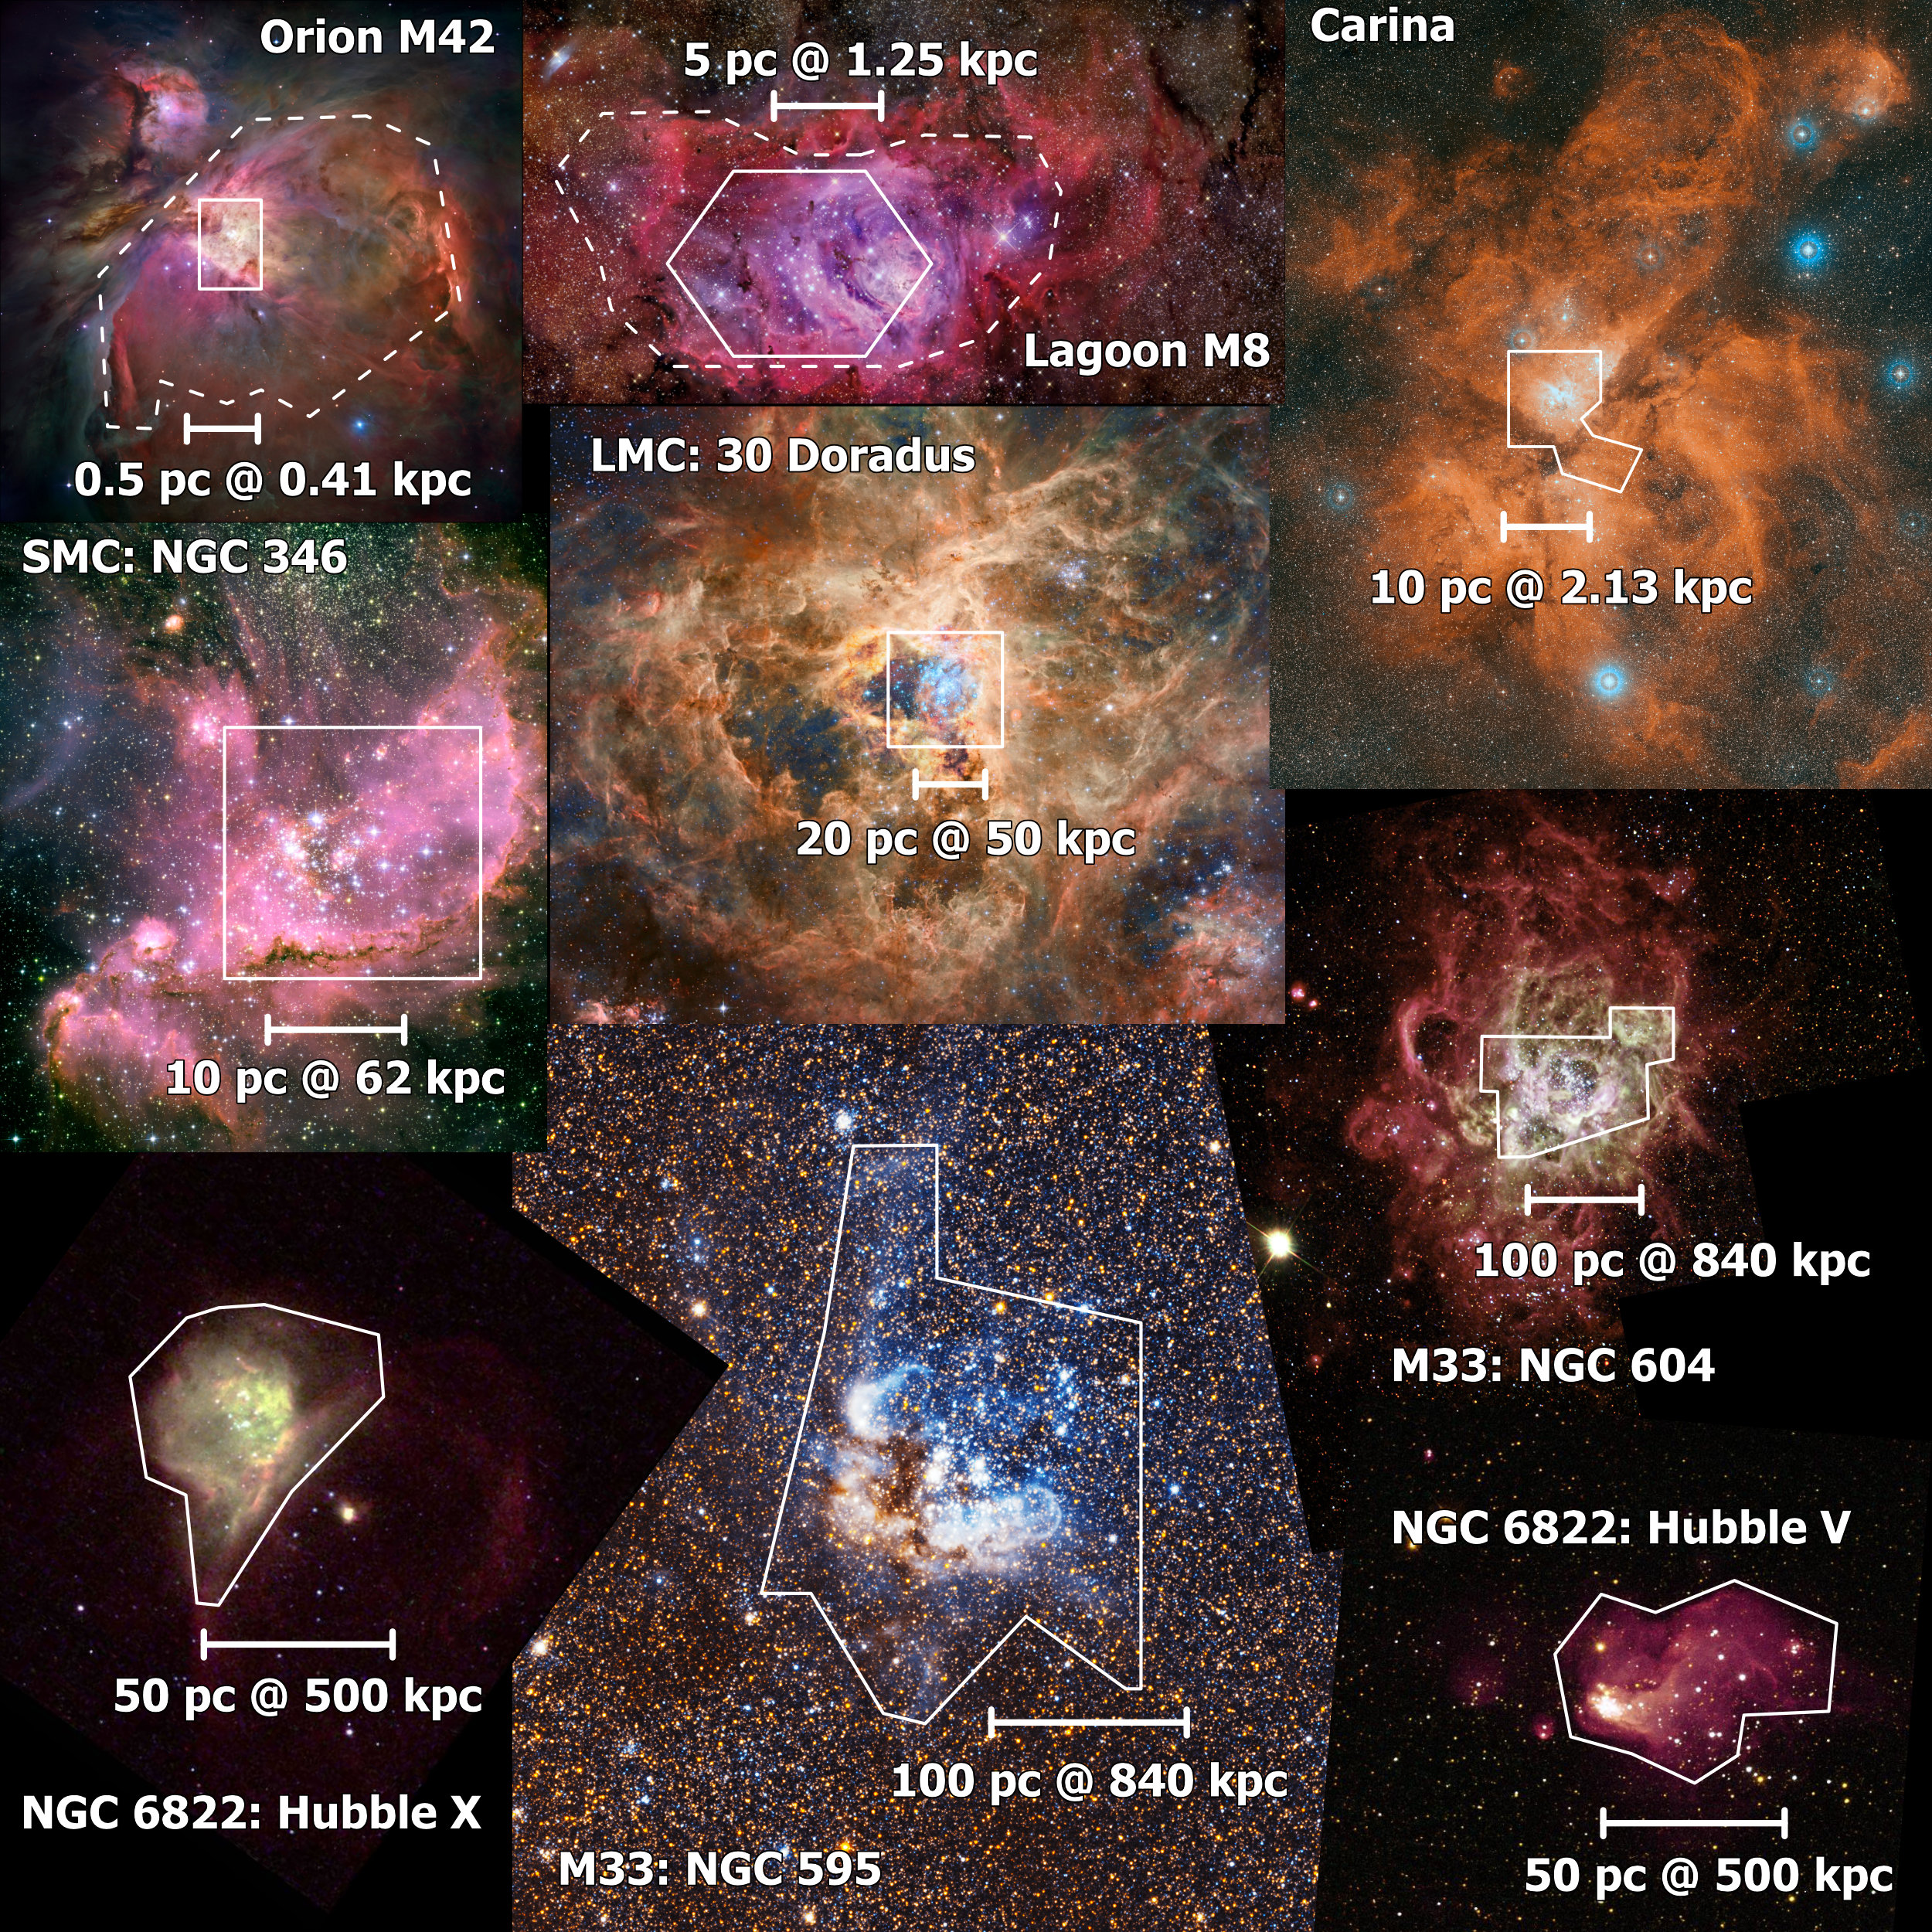
\includegraphics[width=\linewidth]{Figures/hii-region-mosaic}
  \caption{
    The sample of nine \hii{} regions employed in this study,
    arranged from top to bottom in order of distance.
    White shapes show the approximate extents of the
    emission line maps that we use for studying the ionized gas kinematics.
    Scale bars show the equivalent linear length scales at the distance to each region.
    For Orion, two fields are shown: the Extended Orion Nebula,
    sampled at a scale of \SI{0.1}{pc}, and the central Huygens region,
    sampled at a scale of \SI{0.004}{pc}.
    All images are combinations of optical narrow-band and wide-band filters.
    In most cases, red/orange/pink represents \ha{} or other emission lines
    emitted by the ionized gas,
    while blue/white represents continuum starlight from young high-mass stars.
    In some cases, green (for Hubble~X and NGC~604) or blue (for NGC~595)
    represents the [\ion{O}{3}] \Wav{5007} emission line.
    \textit{Image credits as follows.}
    \textbf{Orion Nebula}:
    \textit{HST} Treasury Program on the Orion Nebula Cluster \citep{Robberto:2013a}.
    \textbf{M8 Lagoon}: \href{https://www.cosmotography.com/index.html}{R.~Jay Gabany}.
    \textbf{Carina}: \href{https://www.eso.org/public/images/eso0905b}{
      ESO/Digitized Sky Survey~2, Davide De Martin}.
    \textbf{NGC~346}:
    NASA, ESA and A. Nota (ESA/STScI) \citep{Nota:2006x}.
    \textbf{30 Doradus}:
    \href{http://www.robgendlerastropics.com/Tarantula-HST-ESO.html}{
      Robert Gendler, Roberto Colombari,
      Hubble Legacy Archive, European Southern Observatories}.
    \textbf{Hubble~X}:
    \href{https://hubblesite.org/contents/media/images/2001/01/1012-Image.html}
    {C. R. O'Dell (Vanderbilt University),
      NASA and The Hubble Heritage Team (STScI/AURA)}.
    \textbf{Hubble~V}:
    \href{https://hubblesite.org/contents/media/images/2001/39/1126-Image.html}
    {C. R. O'Dell (Vanderbilt University)
      and L. Bianchi (Johns Hopkins University and Osservatorio Astronomico, Torinese, Italy),
      NASA, ESA, and The Hubble Heritage Team (STScI/AURA)}.
    \textbf{NGC~595}:
    \href{https://esahubble.org/images/heic1901c/}
    {NASA, ESA,
      and M. Durbin, J. Dalcanton, and B. F. Williams (University of Washington)}.
    \textbf{NGC~604}:
    \href{https://hubblesite.org/contents/media/images/2003/30/1423-Image.html}
    {NASA and The Hubble Heritage Team (AURA/STScI)}.
  }
  \label{fig:hii-regions}
\end{figure*}

\begin{figure*}
  \centering
  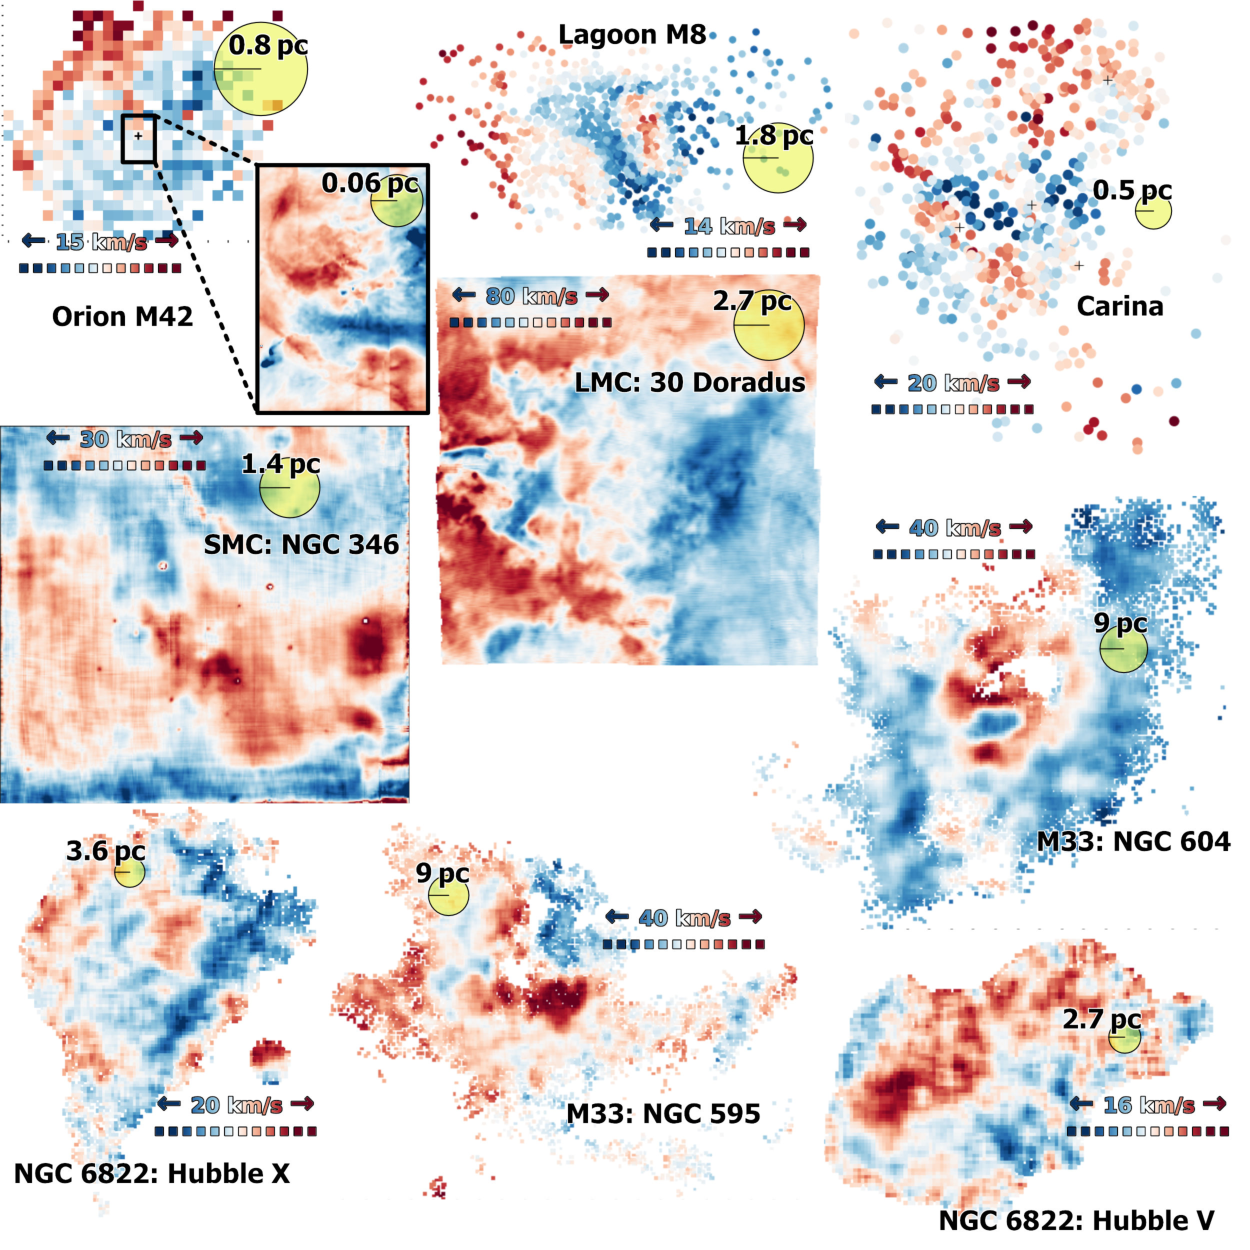
\includegraphics[width=\linewidth]{Figures/velocity-maps-mosaic}
  \caption{
    Maps of the mean \ha{} velocity for each of the regions in our sample.
    All velocities are relative to the systemic velocity of each region,
    with more negative velocities shown in blue and more positive velocities in red.
    The range of velocities is different for each region, as indicated on the individual maps.
    The correlation length of the velocity fluctuations in each region
    is shown as the radius of a yellow circle and labeled with its value in parsecs. 
  }
  \label{fig:velocity-maps}
\end{figure*}

Previous investigations of the centroid velocity structure function in \hii{} regions
have used a variety of methodologies, which makes it difficult to compare results
between different regions.  \citet{arthur2016turbulence} summarise historical results
for the Orion Nebula in their Table~5.
The most significant differences are seen when different emission line tracers are used,
but even when using the same line, there is some variance between different studies
in the derived values for both the velocity dispersion \(\sigma\pos\) and power-law slope \(m\).
It is therefore worthwhile to employ a uniform approach across a variety of different regions.
To that end, we have selected 9 \hii{} regions,
covering a broad range in size and luminosity,
for which good quality mapping of the \ha{} line exists in the literature
or in data archives.
Figure~\ref{fig:hii-regions} shows optical images of
each region in our sample
and Table~\ref{tab:Reg} lists their most important physical parameters.
The derived centroid \ha{} velocity maps are shown in Figure~\ref{fig:velocity-maps}.
Our sample includes three Milky Way regions
(at approximate distance of \num{0.5} to \SI{2}{kpc}),
two regions in the Magellanic Clouds (\num{50} to \SI{60}{kpc}),
and four regions in more distant galaxies of the Local Group
(\num{500} to \SI{800}{kpc}).
Further details of the observations and the sources themselves
are given in the following two sections.

\subsection{Spectroscopic datasets}

%We use data from \citet{1987A&A...176..347H} and \citet{arthur2016turbulence} to study of turbulence in the Orion Nebula.
%\cite{1987A&A...176..347H} observations were obtained using a 106 cm-Cassegrain telescope at Observatorium Hoher List. 
%A Fabry-Pérot interferometer was used with a étalon a separation of 0.5 mm. 
%Interferograms have been taken with different pointing directions of the telescope's optical axis in the nebula. 
%The exposures are overlapped and fall into one square of a grid with a width of 1' centered at \(\theta^{1}\)Ori C.

Wherever possible, we calculate the centroid velocity directly as the first moment
of the line intensity profile for each position on the nebula.
So long as the signal-to-noise is high enough,
this mean velocity can be calculated to a much higher precision
than the nominal velocity resolution of the spectrograph. 
In a few cases, as noted below, we are working with already reduced data,
which are provided in the form of Gaussian fits to the line profiles.
In the cases where multiple Gaussian components have been fitted,
we take the flux-weighted mean velocity of these components to be the centroid.

\subsubsection{Longslit echelle spectroscopy}
\label{sec:longsl-echelle-spect}

For the Orion Nebula, we use data obtained with the echelle spectrograph attached to the \SI{4}{m} telescope at Kitt Peak National Observatory (KPNO) initially published in
\citet{Doi:2004a}.
These observations cover a \(\SI{3}{arcmin} \times \SI{5}{arcmin}\) region of the
central (Huygens) part of the Orion Nebula.
The data consist of 96 North--South orientated \SI{300}{arcsec} slits,
uniformly spaced at \SI{2}{arcsec} intervals with a width of \SI{0.8}{arcsec}
with a velocity resolution of \SI{8}{km.s^{-1}}. 
For the centroid velocities, we use the intensity-weighted
mean velocities calculated by \citet{Garcia-Diaz:2008a},
who used additional observations with East--West oriented slits
to refine the inter-slit velocity calibration. 
Unlike in the previous analysis of this dataset by \citet{arthur2016turbulence},
we do not mask out regions affected by known high-velocity outflows.
This decision was made for consistency with the analysis of more distant regions,
where such a masking out is not possible.

\subsubsection{FLAMES multi-fiber spectroscopy}
\label{sec:flames-multi-fiber}

Archival data from \citet{Damiani:2016a} and \citet{Damiani:2017b} are used
to study the Carina Nebula and Lagoon Nebula, respectively.
These were obtained as a by-product of a study of young stars in their respective regions
as part of the Gaia-ESO Spectroscopic Survey \citep{Gilmore:2012v, Randich:2013m}
using VLT/FLAMES with the GIRAFFE and UVES spectrographs \citep{2002Msngr.110....1P}.
The spectra are from multiple discrete fiber positions in each nebula
(866 positions in Carina; 1089 in the Lagoon),
visible as colored disks in Figure~\ref{fig:velocity-maps}.
The angular separation between fibers varies across the maps with
average nearest-neighbor distance of \SI{21 \pm 17}{arcsec}.
The spectral resolution ranges from  \SI{6}{km.s^{-1}} (UVES) to \SI{16}{km.s^{-1}} (GIRAFFE).
We do not have access to the individual spectra, but instead use the
Gaussian fits to the line profiles from \citep{Damiani:2016a, Damiani:2017b},
obtained from data tables downloaded from the CDS Vizier service.\footnote{%
  \url{https://doi.org//10.26093/cds/vizier.35910074} and
  \url{https://doi.org//10.26093/cds/vizier.36040135}.}
For the Lagoon, we use single-Gaussian fits, while for Carina we take the
flux-weighted mean of the blue and red component of two-Gaussian fits.


\subsubsection{MUSE integral field spectroscopy}
\label{sec:muse-integral-field}

For the Magellanic Cloud regions 30~Doradus and NGC~346 we use data obtained
with the MUSE spectrograph \citep{Bacon:2010a, Bacon:2014a} on the VLT.\@
Each exposure consists of a \(300 \times 300\) pixel spectral image with a plate scale
of \SI{0.2}{arcsec.pixel^{-1}} and a spectral resolution of \SI{110}{km.s^{-1}}
at \ha{}.
For 30~Doradus, four separate exposures are mosaicked to give a square field of
size \(\SI{2}{arcmin}\) \citep{Castro:2018a}. 
We use centroid velocities of single Gaussian fits to the \ha{} line.\footnote{%
  Data kindly provided by Norberto Castro Rodríguez, priv.~comm.
}
For NGC~346, we use a single field that was observed in 2016 as part of
ESO observing program 098.D-0211(A) (P.I. W.-R.~Hamann).
We obtained the pipeline-reduced data cubes from the ESO data archive\footnote{%
  \url{http://archive.eso.org/wdb/wdb/eso/eso_archive_main/query?prog_id=098.D-0211(A)}
}
and extracted the \ha{} profile using tools in the MPDAF python library.\footnote{
  \url{https://mpdaf.readthedocs.io/en/latest/}
} 

\subsubsection{TAURUS-II Fabry-Perot spectroscopy}
\label{sec:taurus-ii-fabry}

The archival data used in this work for the extragalactic giant regions, NGC 604, NGC 595, Hubble X and Hubble V was obtained with the Fabry Perot TAURUS-II instrument
\citep{Gordon:2000v}
on the \SI{4.2}{m} William Herschel Telescope (WHT) of
el Roque de los Muchachos Observatory (ORM) in La Palma, Spain
and was retrieved from the La Palma archive\footnote{\url{http://casu.ast.cam.ac.uk/casuadc/ingarch}}.
Each velocity image is \(256 \times 256\) pixels on the sky,
with a spatial scale of \SI{0.26}{arcsec.pixel^{-1}}
and a spectral resolution of \SI{40}{km.s^{-1}}.
The NGC~604 observations were previously reported and analysed in
\citet{sabalisck1995supersonic}, \citet{Medina-Tanco:1997a} and \citet{Melnick:2021x}.

% \citet{sabalisck1995supersonic} mentioned the main aspects of the observations (1990 July 31).
% The two-dimensional imaging spectroscopy was captured using an IPCS-II detector and the 125 $\mu$m etalon.
% The cumulative integration time per frame is 36 s with a seeing value of 1''.
% The format of the data cube was of 256*256*100 with a spatial scale of 0.26 pixel$^{-1}$.
% Finally, the reduction and analysis was done with the packages TAUCAL y TAUFITS \citep{1992ASPC...25..445L}. The NGC 604 TAURUS-II observations were used by \citet{sabalisck1995supersonic}, \citet{tanco1997} and \citet{2019arXiv191203543M}.


\subsection{Physical properties of the sample regions}
\label{sec:regions-milky-way}

\begin{table}
\begin{center}\caption{Summary of properties of our \hii{} region sample}
\begin{tabular}{l CCCC}\toprule
\hii{}    &  \text{Distance,}\ D& \text{Diameter,}\ R & \log L(\ha) &  \langle \sigma\los \rangle \\
  Region    &  [\si{kpc}]          &  [\si{pc}]    &  [\si{erg.s^{-1}}]            &    [\si{km.s^{-1}}]  \\ 
\midrule
Orion    & 0.436 \pm 0.02  & 0.6 \pm 0.06  &    37               &   6.0      \\
%Orion large   & 0.436 \pm 0.02  & 5 \pm 0.5    &    37               &   6.0      \\ 
Lagoon    & 1.25 \pm 0.12   & 25 \pm 2.5       &    37.47            &   13.6     \\
Carina    & 2.35 \pm 0.05   & 15 \pm 1.5       &    39.6             &   22.4     \\
30 Dor    & 50.0 \pm 0.2  & 98.9 \pm 9.8     &    39.76            &   31.7     \\
NGC 346   & 62 \pm 1    & 64 \pm 6.4       &    38.67            &   10.2     \\
Hubble X  & 490 \pm 40      & 160 \pm 16      &    38.6             &   13.4     \\
Hubble V  & 490 \pm 40      & 130 \pm 13 &    38.87            &   12.3     \\
NGC 604   & 820 \pm 30      & 400 \pm 40      &    39.65            &   16.2     \\
NGC 595   & 820 \pm 30      & 400 \pm 40      &    39.36            &   18.3     \\
\bottomrule
\end{tabular}\label{tab:Reg}
\end{center}
\end{table} 

\subsubsection{Orion Nebula}
\label{sec:orion-nebula}

Orion (M42) is the prototype galactic HII region and one of the mores studied in the sky.
Located at a distance of 440 pc \citep{2008AJ....136.1566O} its main physical and kinematics properties, along its stellar population are documented in \citet{2001ARA&A..39...99O}.
The main ionizing star is \(\theta^{1}\)Ori C (spectral type \(\sim\)O7) and with other 3 B-type stars they form the Trapezium cluster.
The position of Orion near the side of the Orion Molecular Cloud (OMC-1) make it an ongoing star formation region and a example of a blister HII region. Some of these young stars are accountable for stellar jets and Herbig-Haro objects seen in the nebula \citep{arthur2016turbulence}.

\subsubsection{Carina Nebula}
\label{sec:carina-nebula}

The Carina nebula is a large star-forming complex located at a distance of 2 350 pc \citep{2006ApJ...644.1151S}.
Young clusters like Trumpler 14 and 16, and Collinder 228 together form the Car OB1 association.
This OB association has more than 65 stars earlier than B0, and several Wolf-Rayet stars.
The most star is a luminous blue variable, $\eta$ Car \citep{Damiani:2016a}.
As a star formation region, it presents several phenomena related with young stars as evaporating protoplanetary discs, erosion of large dust pillars and the triggering of a second generation of embedded stars, Herbig-Haro objects, to mention some, \citet{2008hsf2.book..138S} and reference therein.
An approaching and receding kinematics components are known in the nebula.

\subsubsection{Lagoon Nebula}
\label{sec:lagoon-nebula}


The Lagoon Nebula (M8, NGC6523) is located at a distance of 1 250 pc \citep{2005A&A...430..941P} and contains the young stellar cluster NGC6530.
The region is illuminated by different massive stars of spectral types O and B, the hottest being 9 Sgr, type O4V \citep{Damiani:2017b}.
Optically, the brightest part of the nebula is called 'Hourglass nebula' which surrounds and obscures the star Herschel 36, type O7 \citep{1986AJ.....91..870W}. 
The velocity field shows several expanding shells, related to the cluster NGC 6530, the O stars 9 Sgr and Herschel 36, and the massive protostar M8East-IR. A blueshifted, neutral layer is also in very good agreement with predictions of champagne-flow models of blister HII regions \citep{Damiani:2017b}. The properties of the nebula are reviewed by \citet{2008hsf2.book..533T}.

\subsubsection{30 Doradus}
\label{sec:30-doradus}

The Tarantula Nebula (30 Doradus) is a luminous star-forming region in the LMC (Large Magellanic Cloud) and is the most luminous complex in the Local Group \citep{1984ApJ...287..116K}. The nebula is located at a distance of 49.9 kpc \citep{2013Natur.495...76P}.
It host the star forming region NGC 2070 that contains the massive star cluster R136. 
The star formation rate gas increased recently, 1-3 Myr ago \citep{2016ApJ...833..154C}, and the central ionized region spans for 40 pc.
This nebula is used as a comparison for extragalactic star-forming regions.

\subsubsection{NGC 346}
\label{sec:ngc-346}


NGC 346 is the most active star-formation region in the SMC (Small Magellanic Cloud) located at a distance of 62 kpc \citep{2001ApJ...562..303D}. 
It has more than 30 O stars that ionize N66, the largest HII region \citep{2011ApJ...740...10D}.
\citet{2008ApJ...688.1050G} propose an expanding H II region or bubble blown by the winds of the massive progenitor as a mechanism that shapes the recent star formation in this region in addition to the photoionizing process of the OB stars. 
This mechanism is similar to shell-like H ii regions, with a central cluster in a cavity, and with ongoing star formation triggered around their periphery.

\subsubsection{Hubble X and Hubble V in NGC 6822}
\label{sec:hubble-x-hubble}


The dwarf irregular galaxy, NGC 6822, is located at a distance of 500 kpc (1'' = 2.4 pc) \citep{2012A&A...540A.135S} and the brightest HII regions are Hubble X and Hubble V (HX and HV hereafter).
HV has a characteristic length of 100 pc and a luminosity at its core of in L$_{H_\alpha}$ = 1 $\times$ 10$^{49}$ H$\alpha$ photons s$^{-1}$ \citep{1999PASP..111.1382O}.
HX has a characteristic length of 140 pc and a luminosity at its core of in L$_{H_\alpha}$ = 2.4 $\times$ 10$^{49}$ H$\alpha$ photons s$^{-1}$ \citep{1999PASP..111.1382O}.
Two recognized OB associations \citep{1991ApJ...379..621H,1992AJ....104.1374W} are identified within the region of HV and HX. HV is located near 'Hodge OB 8', and HX is located near 'Hodge OB13'  \citep{1999PASP..111.1382O}.


\subsubsection{NGC~595 and NGC~604 in M33}
\label{sec:ngc-595-ngc}

NGC 604 is the brightest giant HII region in the M33 galaxy visually dominated by a big loop, many shells and different size filaments.
It is located at the distance of 840 kpc (1'' = 4.1 pc) \citep{2015KamKinematics} with a length of 400 pc.
It has a luminosity in L$_{H_\alpha}$ = 10$^{39.42}$ erg s$^{-1}$ \citep{2002MNRAS.329..481B} and in L$_{X}$=9.3$\times$ 10$^{35}$ erg s$^{-1}$ \citep{2008ApJ...685..919T}.
\citet{2012ApJ...761....3M} derive an average age of 4$\pm$1 Myr and a total stellar mass of 1.6$^{+1.6}_{-1.0} \times$ 10$^{5}$M$_{\odot}$ for the region.
The stellar population has been identified and classified by \citet{1996ApJ...456..174H} (and references therein).
Recently, \citet{2011MNRAS.411..235E} focused on studying the Wolf-Rayet (WR) and red super giants (RSGs) stars population.
\citet{2012AJ....143...43F} focused on the massive young stellar objects (MYSOs).
The average ages for the stars, was determined to be from 3 to 5 Myr \citep{1996ApJ...456..174H} and with the RSGs as an older population have an age of 12.4 $\pm$ 2.1 Myr \citep{2011MNRAS.411..235E}.
This suggest that two episodes of star formation, at least, have taken place in the GEHR.
%\citep{1984A&A...141...49H} identified a gradient from the west to the SE of the nebula of 30 km s$^{-1}$.

NGC 595 is the second brightest giant HII region in the M33 galaxy.
%The electronic temperature is 7,670 $\pm$116 K \citep{2010MNRAS.402.1635R}.
\citet{1983A&A...119..185V} made an estimate of the total masses of HI and HII in the nebula to obtain values of M$_{HI}=$ 1.2 $\times$ 10 $^{6}$ M$_{\odot}$ and M$_{HII} =$ 4.6 $\times$ 10 $^{5}$ M$_{\odot}$, and a ionizing luminosity of the star cluster is estimated at 5 $\times$ 10$^{50}$ erg s $^{1}$.
\citet{1996AJ....111.1128M} estimate an age of 4.5 Myrs consistent with \citet{1993AJ....105.1400D}.
It has approximately 250 stars of the OB type, 13 Supergiants and 9 WR \citep{1996AJ....111.1128M}, ten WRs confirmed with spectroscopy \citet{1993AJ....105.1400D}, nine of the WN type and a WC, located near the bright core of the region.



%2013ApJ...773...69G M33 dist
% \citep{1984ApJ...287..116K} \citep{1986ApJ...300..624R}

%%%%%%%%%%%%%%%%%%%%%%%%%%%%%%%%%%%%%%%%%%%%%%%%%%%%%%%%%%%%%%%%%%%%%%%%%%%%%%%%%%%%%%%%%%%%%%%%%%%%
%%%%%%%%%%%%%%%%%%%%%%%%%%%%%%%%%%%%%%%%%%%%%%%%%%%%%%%%%%%%%%%%%%%%%%%%%%%%%%%%%%%%%%%%%%%%%%%%%%%%%%%

\section{Plane-of-sky velocity fluctuations}\label{sec:met}


\subsection{The second-order structure function}
\label{sec:second-order-struct}
One of the fundamental properties of turbulent clouds must be spatial fluctuations in velocity and density.
These fluctuations are observed as projected spatial fluctuations in the average line-of-sight velocity and integrated column density.
It is possible to describe the statistical properties of these fluctuations if they are assumed as a product of a stochastic field \citep{1984ApJ...277..556S}. 
This previous assumption give us the ability to apply statistical tools to the velocity field and the analysis of the velocity pattern is reduced to the calculation of the averages and correlations.

The second-order structure function of the velocity centroids, $B(r)$, is defined as:
%
\begin{equation}\label{eq:Br}
  B(\boldsymbol{r}) = \dfrac{1}{N(\boldsymbol{r})}
  \,
  \sum_{\text{pairs}} \bigl[
  V_{c}(\boldsymbol{x} + \boldsymbol{r}) - V_{c}(\boldsymbol{x})
  \bigr]^{2}
\end{equation}
%
where $N(\boldsymbol{r})$ is the number of pair points at each separation \(\boldsymbol{r}\), called lag. 
In the Kolmogorov model \(B(r) \propto r^{2/3}\).

The variance of the centroid velocity fluctuations is:
%
\begin{equation}\label{eq:variance}
\sigma^2  = \frac{1}{N} \sum_{\text{pixels}} \bigl[ V_c (\boldsymbol{x}) -\langle V_ c\rangle  \bigr]^2
\end{equation}
%
the, \(\langle V_c \rangle \) is the mean centroid velocity
%
\begin{equation}\label{eq:mean}
\langle V_c \rangle \  = \frac{1}{N} \sum_{\text{pixels}} V_c (\boldsymbol{x})
\end{equation}
%
The summation in Equation \ref{eq:Br} is over all data pairs for each separation \(N(\boldsymbol{r})\).
The summations in Equations \ref{eq:variance} and \ref{eq:mean} are over the total number of valid pixels in the (\textit{x},\textit{y})-plane.

\subsection{Application to our HII regions sample}\label{sec:apply}

The autocovariance function is:

\begin{equation}\label{eq:Cr}
C(\boldsymbol{r}) = \dfrac{\sum_{\text{pairs}}[V_{c}(\boldsymbol{x} + \boldsymbol{r}) \times V_{c}(\boldsymbol{x}) ]} {N(\boldsymbol{r})}
\end{equation}
%
and is another statistical tool used in studying the turbulent flows.
The interpretation of the Equation \ref{eq:Cr} depends on the assumption of homogeneity, which may be violated for astrophysical processes.
Because of this, Equation \ref{eq:Br} is a better approach to characterize the velocity fluctuations even in the presence of large scale linear gradients and may be sensitive to a wider range of scales \citep{1984ApJ...277..556S}.

For the homogeneous random field, Equations \ref{eq:Br} and \ref{eq:Cr} are related by:

\begin{equation}\label{eq:functional}
B(r; r_0, m) = 2\sigma^2 \bigl( 1 - C(r) \bigr)
\end{equation}

%Based on Equation \ref{eq:functional} we use the functional of the structure function in the form:
%
%\begin{equation}\label{eq:ff}
%b(r; r_0, m) = 2\sigma^2 \bigl( 1 - C(r) \bigr)
%\end{equation}
%
%where  is now the new form of the correlation function in the form:
where $C(r)$ is a new form that we propose of the correlation function:
%
\begin{equation}\label{eq:ffnew}
  C(r) = \exp \left[ -(\ln 2) \left( \frac{r}{r_0} \right)^m \right]
\end{equation}
%
substituting the previously $C(r)=1/[1+(r/r_{0})^{m}]$ \citep{1966igd..book.....K,1984ApJ...277..556S}.

The term $r_{0}$ is the correlation length of the turbulence, the value of \(r\) in pc where equation \ref{eq:Br} reach the value of \(\sigma^2\), and $m$ is the index that adjust our results.
In this idealized case, at scales larger than r$_{0}$ the structure function flattens as it tends towards the asymptotic value of 2$\sigma$ \citep{arthur2016turbulence}.

The model proposed to describe the seeing at small scales is:
%
\begin{equation}\label{eq:ffs}
  S(r; s_0, r_0) = \frac{
    e^{-s_0 / r_0}
  }{
    1+(2s_0 / r)^{2 / 3}
  }
\end{equation}
%
and the model that consider the effect of the observational box size is:

\begin{equation}\label{eq:ffb}
% \beta(r_0) = 1 - exp[\frac{L_{box}}{3.6r_0}] 
  \beta(r_0) = 1 - \exp \left[ -L_{\text{box}} / (3.6 r_0) \right] 
\end{equation}
%
where $L_{\text{box}}$ is the diagonal length of the observational box.

The final form of our proposed functional of the structure function is in the form:
%
\begin{equation}\label{eq:fff}
B(r) = b(r; \beta r_0, \beta m) \times S(r; s_0, r_0) + B_{\text{noise}}
\end{equation}

The results obtained with equation \ref{eq:Br} are use in a non-linear least-squares
fit to obtain the best values for the turbulent parameters. 
We use equation \ref{eq:fff} in a chi-square analysis applying the equation:
%
\begin{equation}\label{eq:chi}
  \chi^2 = \sum_i ^N \frac{[y_i^{\text{measure}}-y_i^{\text{model}} (\boldsymbol{v})]^2}{\epsilon_i ^2}
\end{equation}
%
using the package \textit{lmfit} \citep{newville_matthew_2014_11813}. 

In this way we avoid one fundamental problem in the interpretation of the structure function results. 
The slope in the majority of previous studies and hence, the correlation length, is obtained without a formal procedure. 
The traditional way to find it is to determine a particular range of ascending values in the structure function results. 
If this increase in values is stopped or reversed it is commonly assumed that one particular inertial range has been found. 
In some cases this procedure keeps going up to large scales, giving two or more inertial regimes leading to the erroneous interpretation of multiple inertial scales.


\subsection{Turbulence}

\textit{Will 2021-12-10: Moving this section to later for now. Maybe
  this material could go in discussion}

The existence of turbulent flows in astrophysical objects, ranging in scales from 10$^{6}$ to 10$^{17}$ m \citep{2010ApJ...710..853C} is the consequence of the high Reynolds numbers, $Re$, between 10$^{4}$ and 10$^{9}$ \citep{1949ApJ...110..329C,lagrois2011} that characterized these objects.
The classic turbulence theory assumes a three-dimensional isotropic, incompressible and subsonic flow that can be described using an energy spectrum \citep{kolm1}.
The concept of the energy spectrum is based on the assumption that the energy is cascading down inside the flow from the largest to the smallest scales.
The different scales in the energy cascade are defined based on their $Re$.
In one side of the spectrum there is the energy, \(L\), injection scale that is related to the largest vortices, where $ Re \rightarrow \infty$.
On the other side of the spectrum there is the dissipation of energy at small scales, \(l\), where $Re \rightarrow$ 1 and it is assumed that small vortices are responsible for the friction that dissipates the energy flux into thermal energy.
In between there is the inertial range, \(l  << r << L\) , where in a stationary case there energy transfer is at a constant rate,.
The energy cascade concept is described with an energy spectrum, $E(k) \propto k^{\beta}$ where $k$ is the wave number for a determined scale $r$ ($k \equiv r^{-1}$).

The total specific energy of a determined $r$ scale is of the order $\langle v_{r}^{2} \rangle$ and is the energy integral above the associated $k$, defined as:
\begin{equation}\label{eq:energyspectrum}
 \langle v_{r}^{2} \rangle = \int_{k}^{\infty} E(k)dk
\end{equation}
%
It is assumed that this energy is of the order of $(\epsilon r)^{\frac{2}{3}} \sim (\frac{\epsilon}{k})^{\frac{2}{3}}$ we differentiate Equation \ref{eq:energyspectrum} and obtained the final form of the spectrum:

\begin{equation}\label{eq:kolm}
E(k) \propto \epsilon^\frac{2}{3} k^{-\frac{5}{3}}
\end{equation}
%
where \(\epsilon\) is the energy transfer rate and the value of $\beta = -5 / 3$ is the Kolmogorov index.
%For supersonic turbulence the index is $\beta=-2$ \citep{burg}. 


\section{Results}\label{sec:results}

\subsection{Data}

The Figure \ref{fig:velocity-maps} shows the velocity maps of each HII region in the \halpha\ emission line.
All velocities are relative to the systemic velocity of each region, with more negative velocities shown in blue and more positive velocities in red. The range of velocities is different for each region and is shown in each map. The more negative velocities are shown in blue and more positive velocities are shown in red.
The Figure \ref{fig:hist} shows the probability density functions of our sample of HII regions.
All the distributions are far from being consider Gaussian, implying that there are multiple kinematics components in the regions.

\begin{figure*}
 \centering
 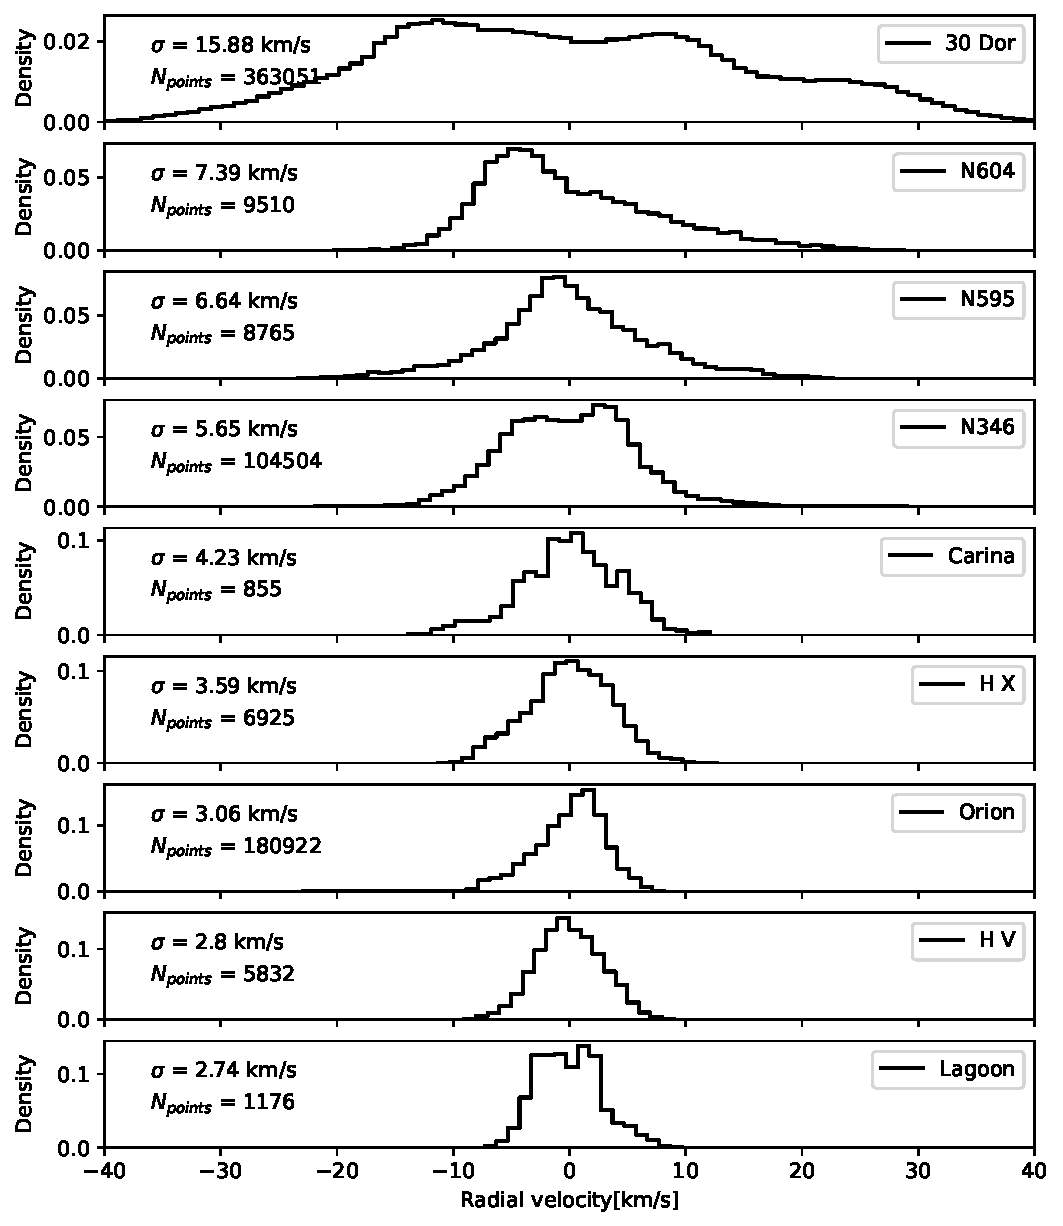
\includegraphics[width=5in]{Figures/Hist/Hist}\par
 \caption{Histograms of the centroid velocities in \halpha\ of our sample of HII regions. }
 \label{fig:hist}
\end{figure*}

\subsection{HII regions structure functions}

Figures \ref{fig:strucfunc-fit-A}-\ref{fig:strucfunc-fit-C} shows the structure function of each region along with the fit obtained using the non-linear regression.
Table \ref{tab:Res} presents the turbulent parameters we obtain the regression.
The second column correspond to the variance \(\sigma^2\) of the velocity field.
The index \(m\) is shown in the third column and is used as a reference for comparison between theory and observations.
The fourth column is the correlation length \(r_0\).

\begin{figure*}
  \centering
  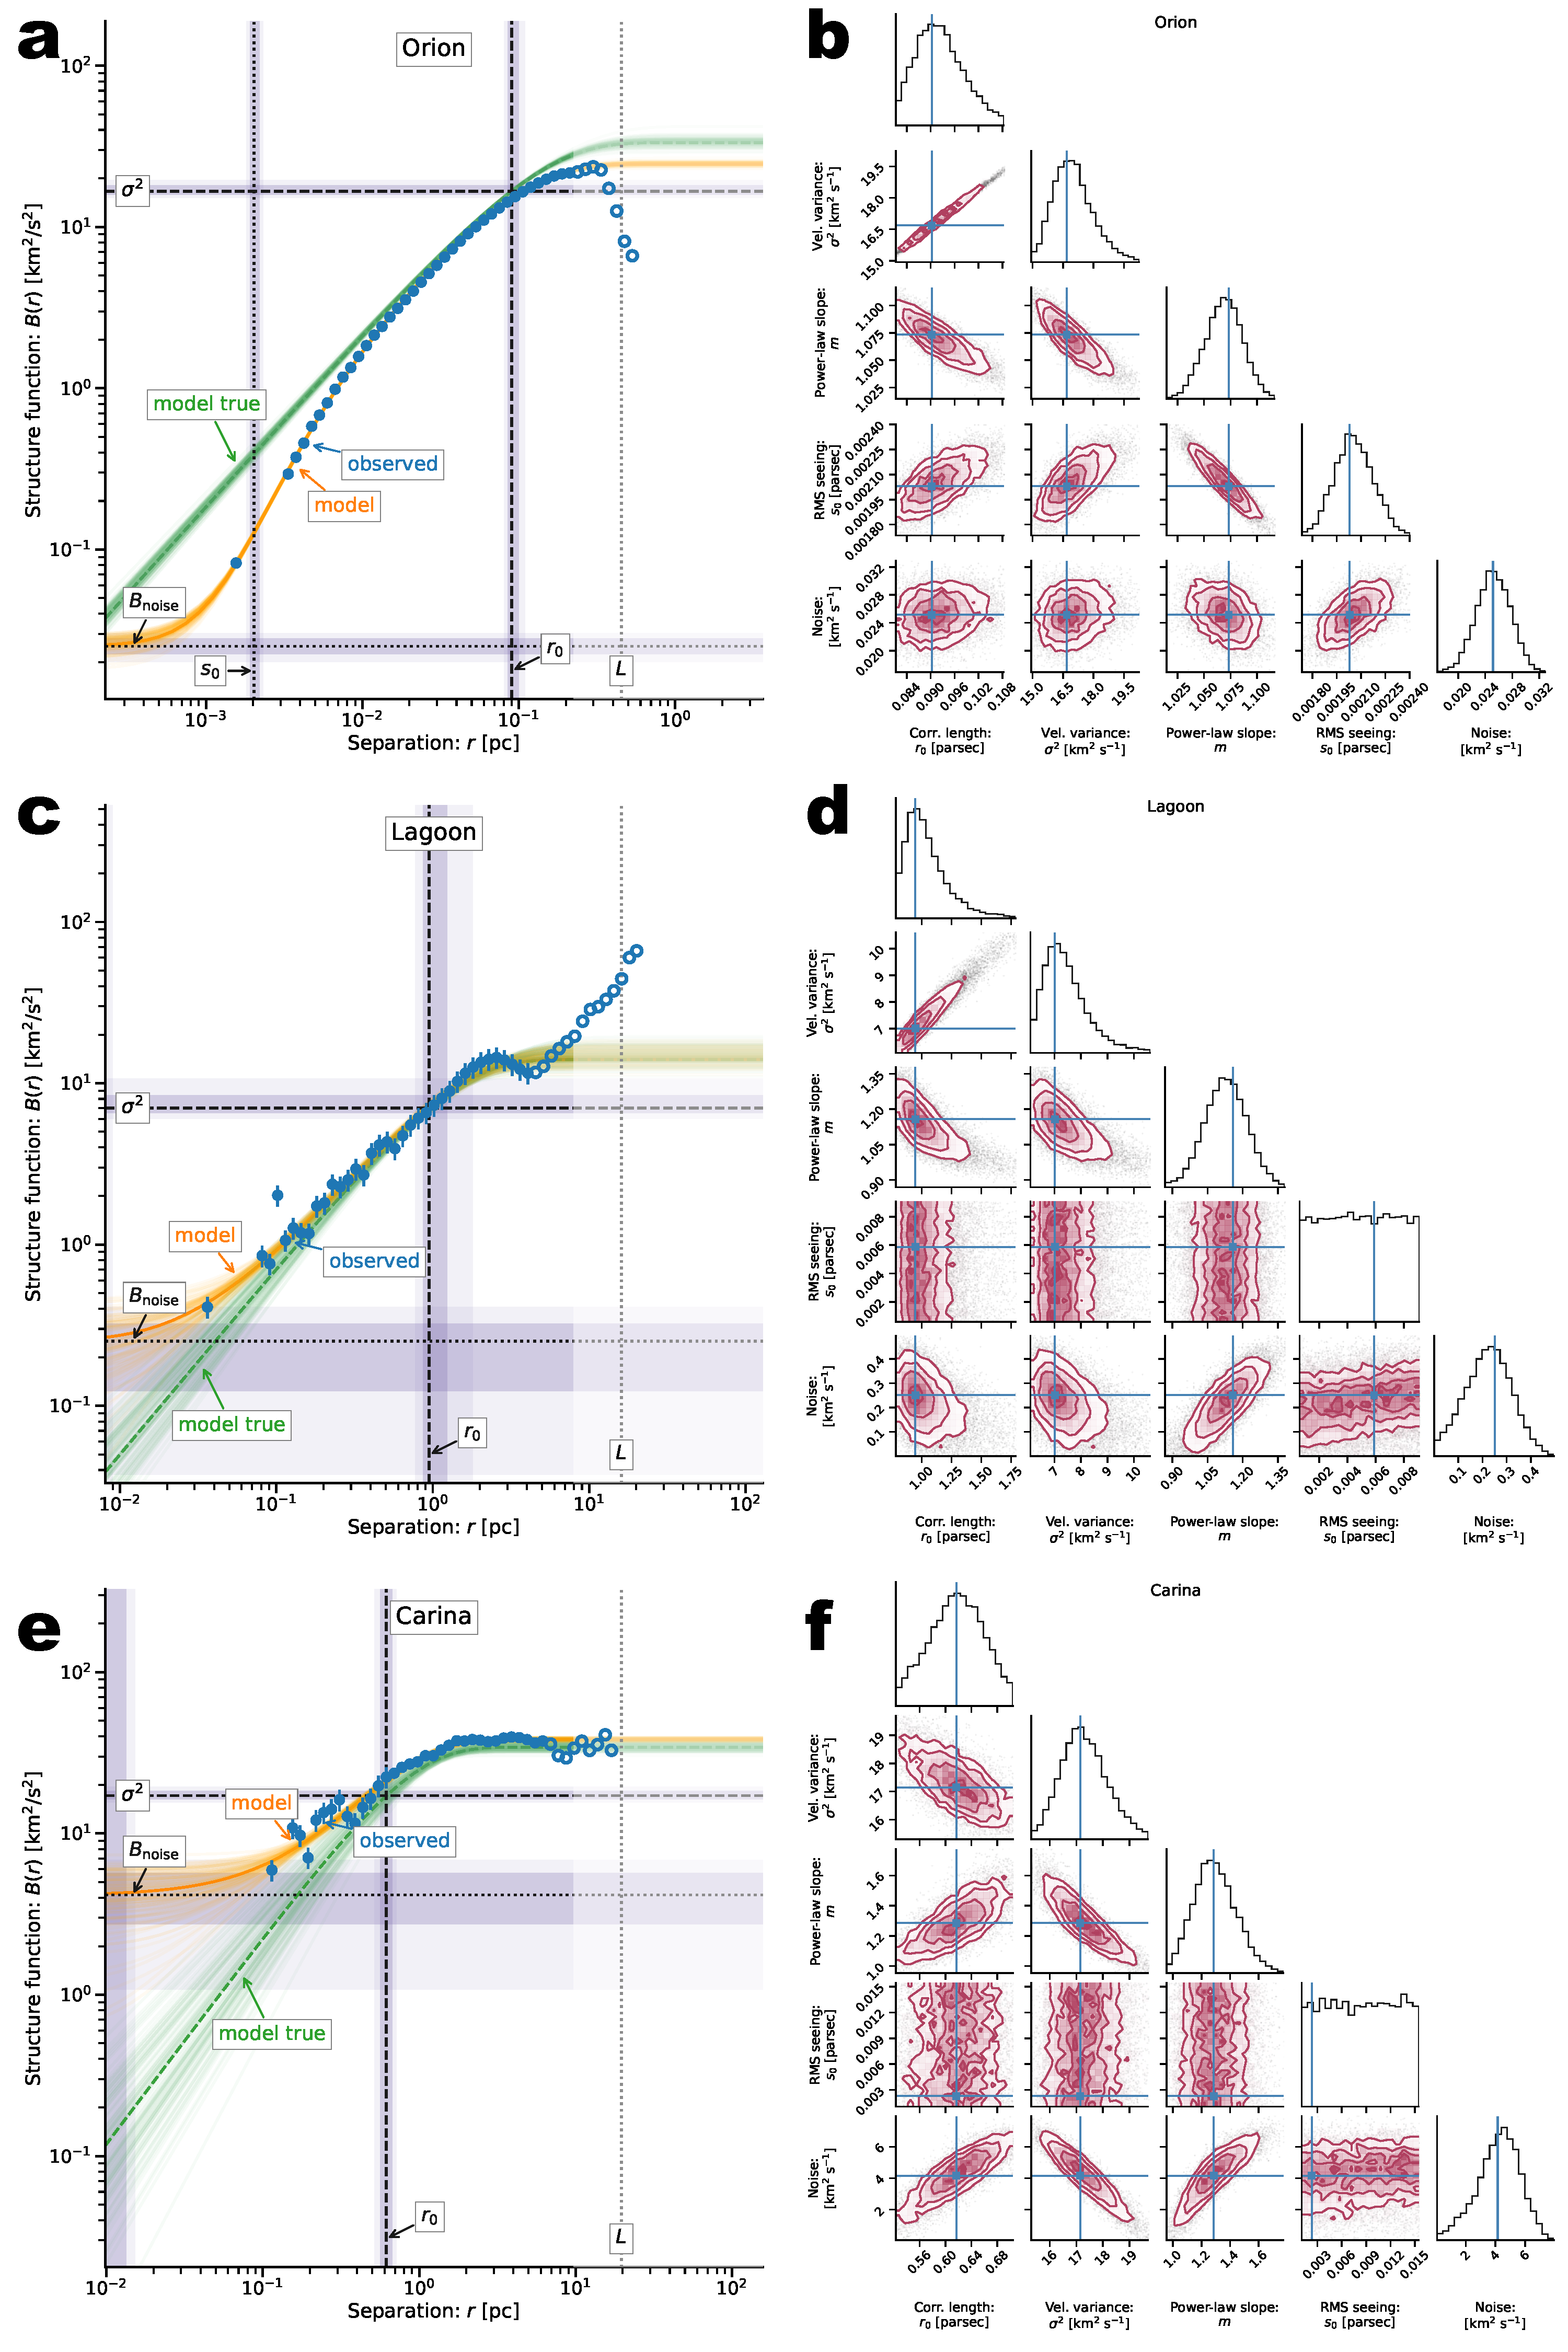
\includegraphics[width=0.8\linewidth]{Figures/strucfunc-fit-A}
  \caption{Second-order structure functions for the velocity centroid images of the \(H\alpha\) emission line}\label{fig:strucfunc-fit-A}
\end{figure*}

\begin{figure*}
  \centering
  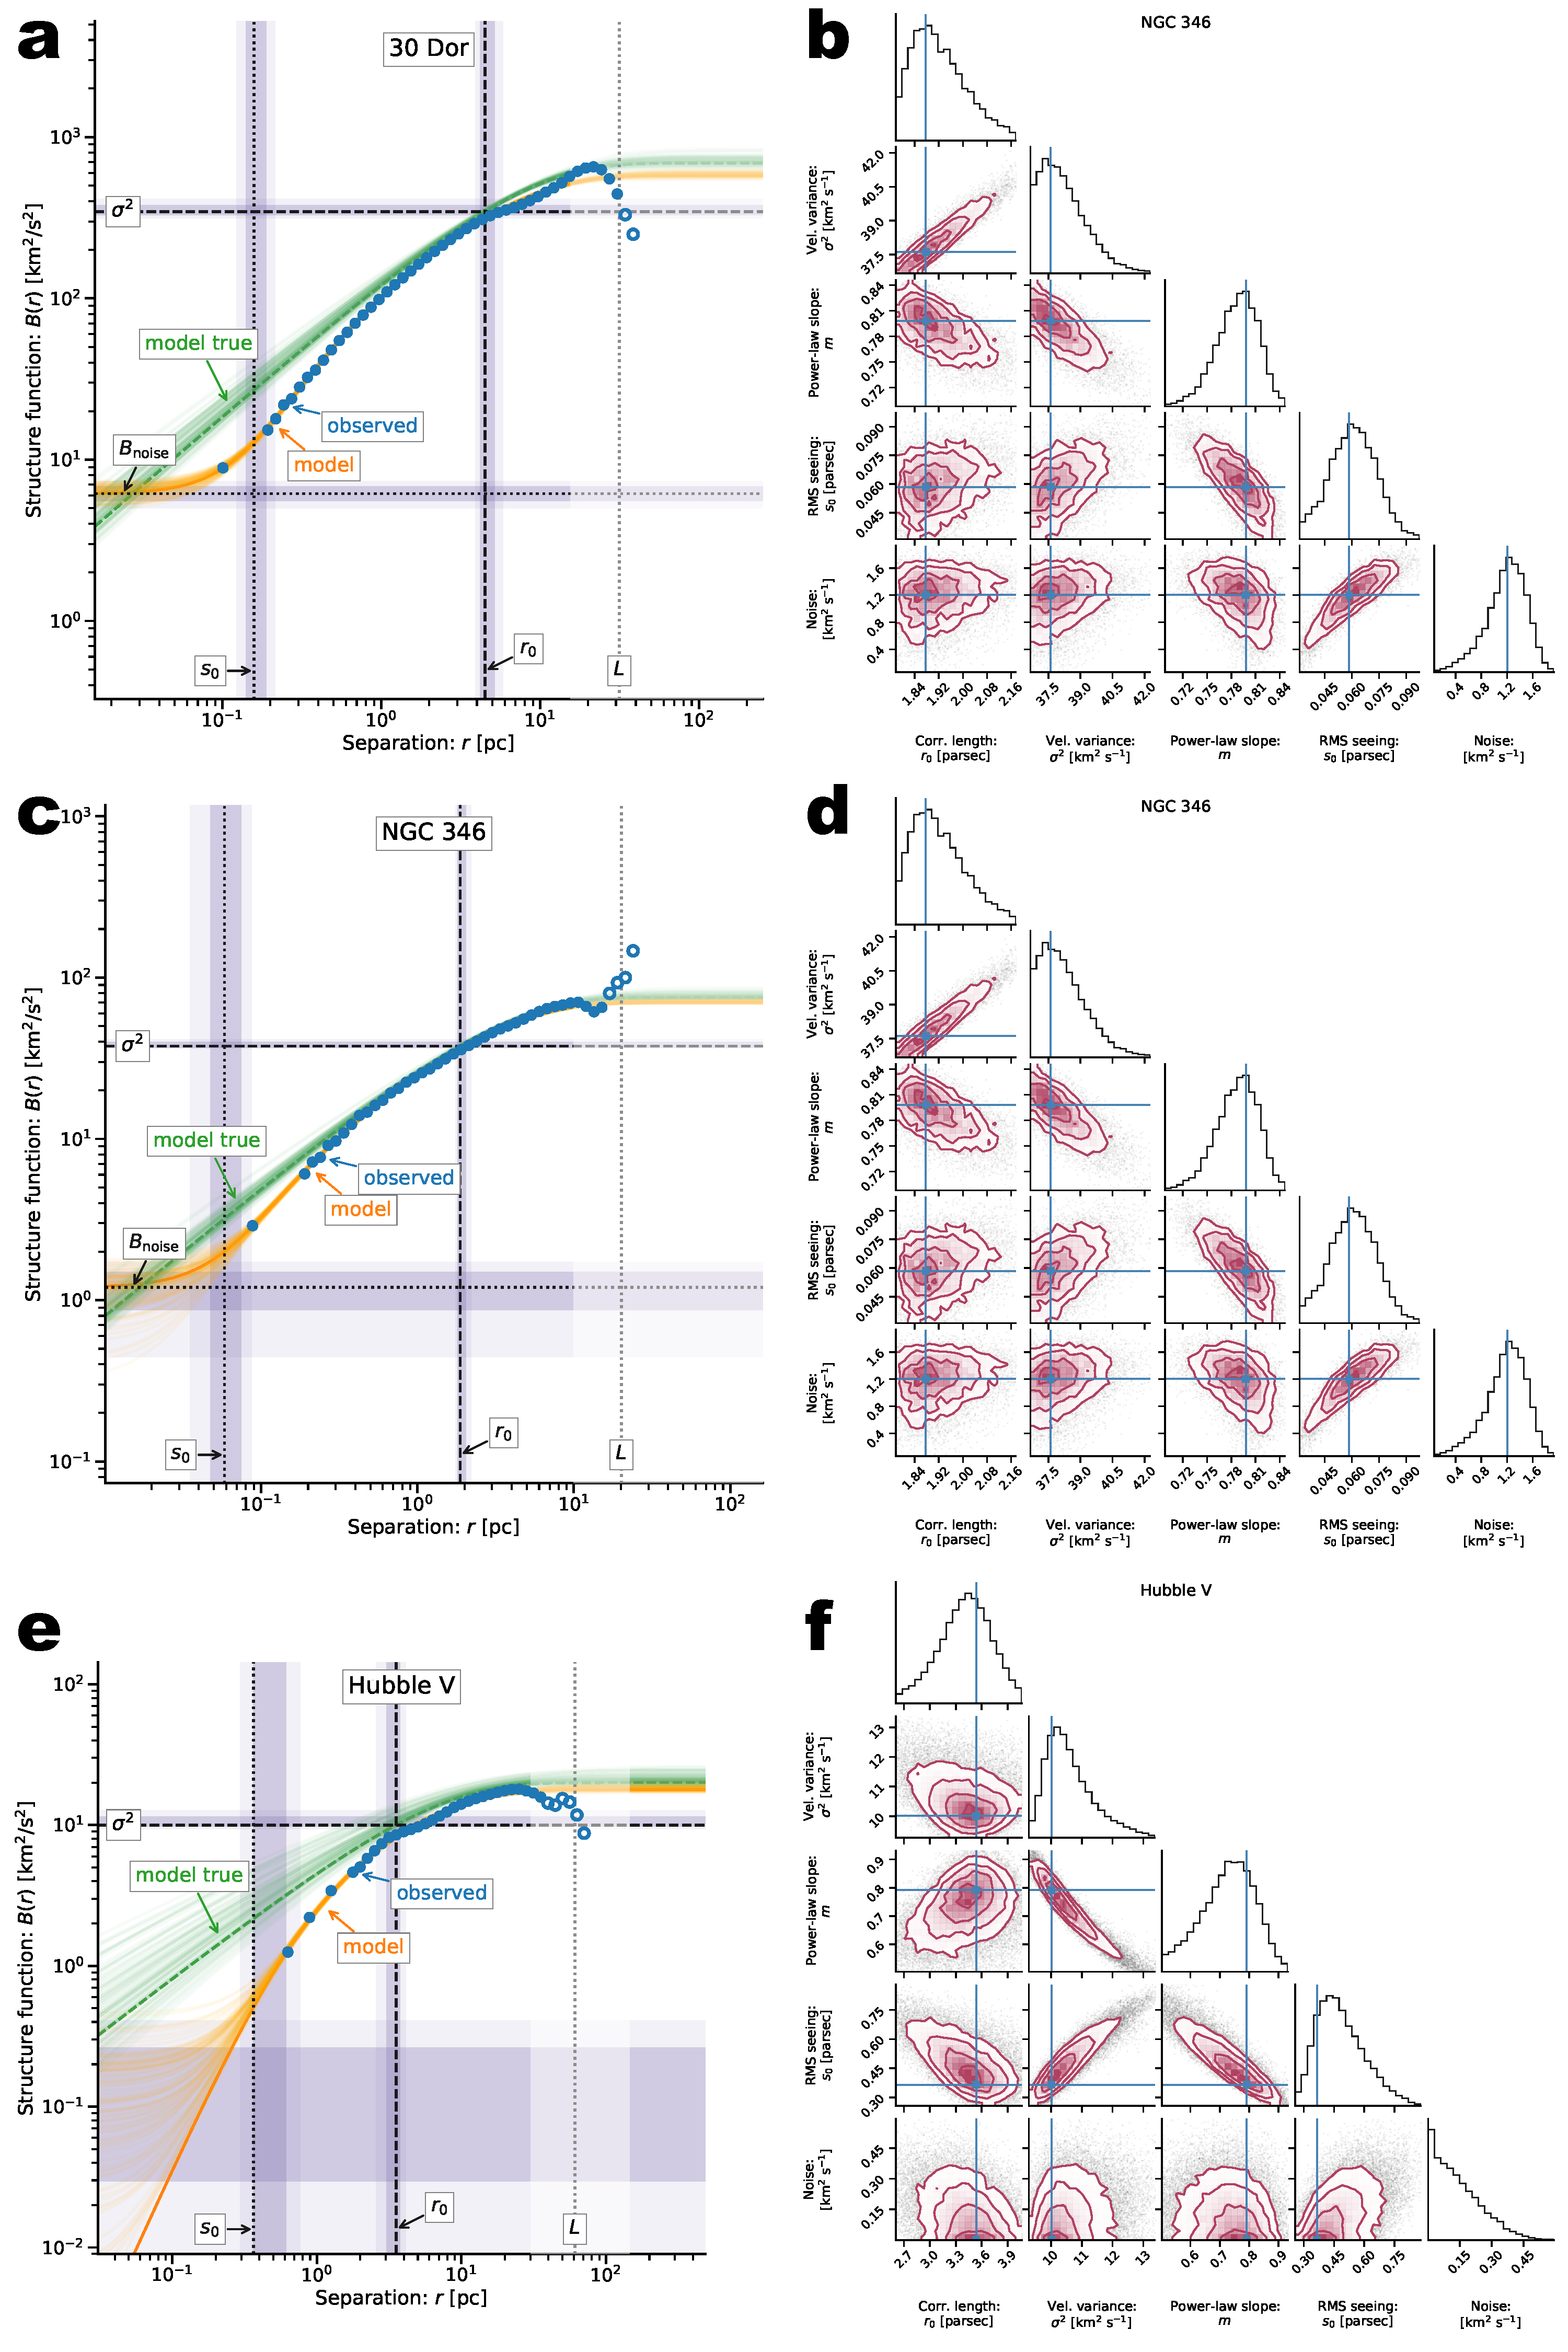
\includegraphics[width=0.8\linewidth]{Figures/strucfunc-fit-B}
  \label{fig:strucfunc-fit-B}
  \caption{Second-order structure functions for the velocity centroid images of the \(H\alpha\) emission line}
\end{figure*}

\begin{figure*}
  \centering
  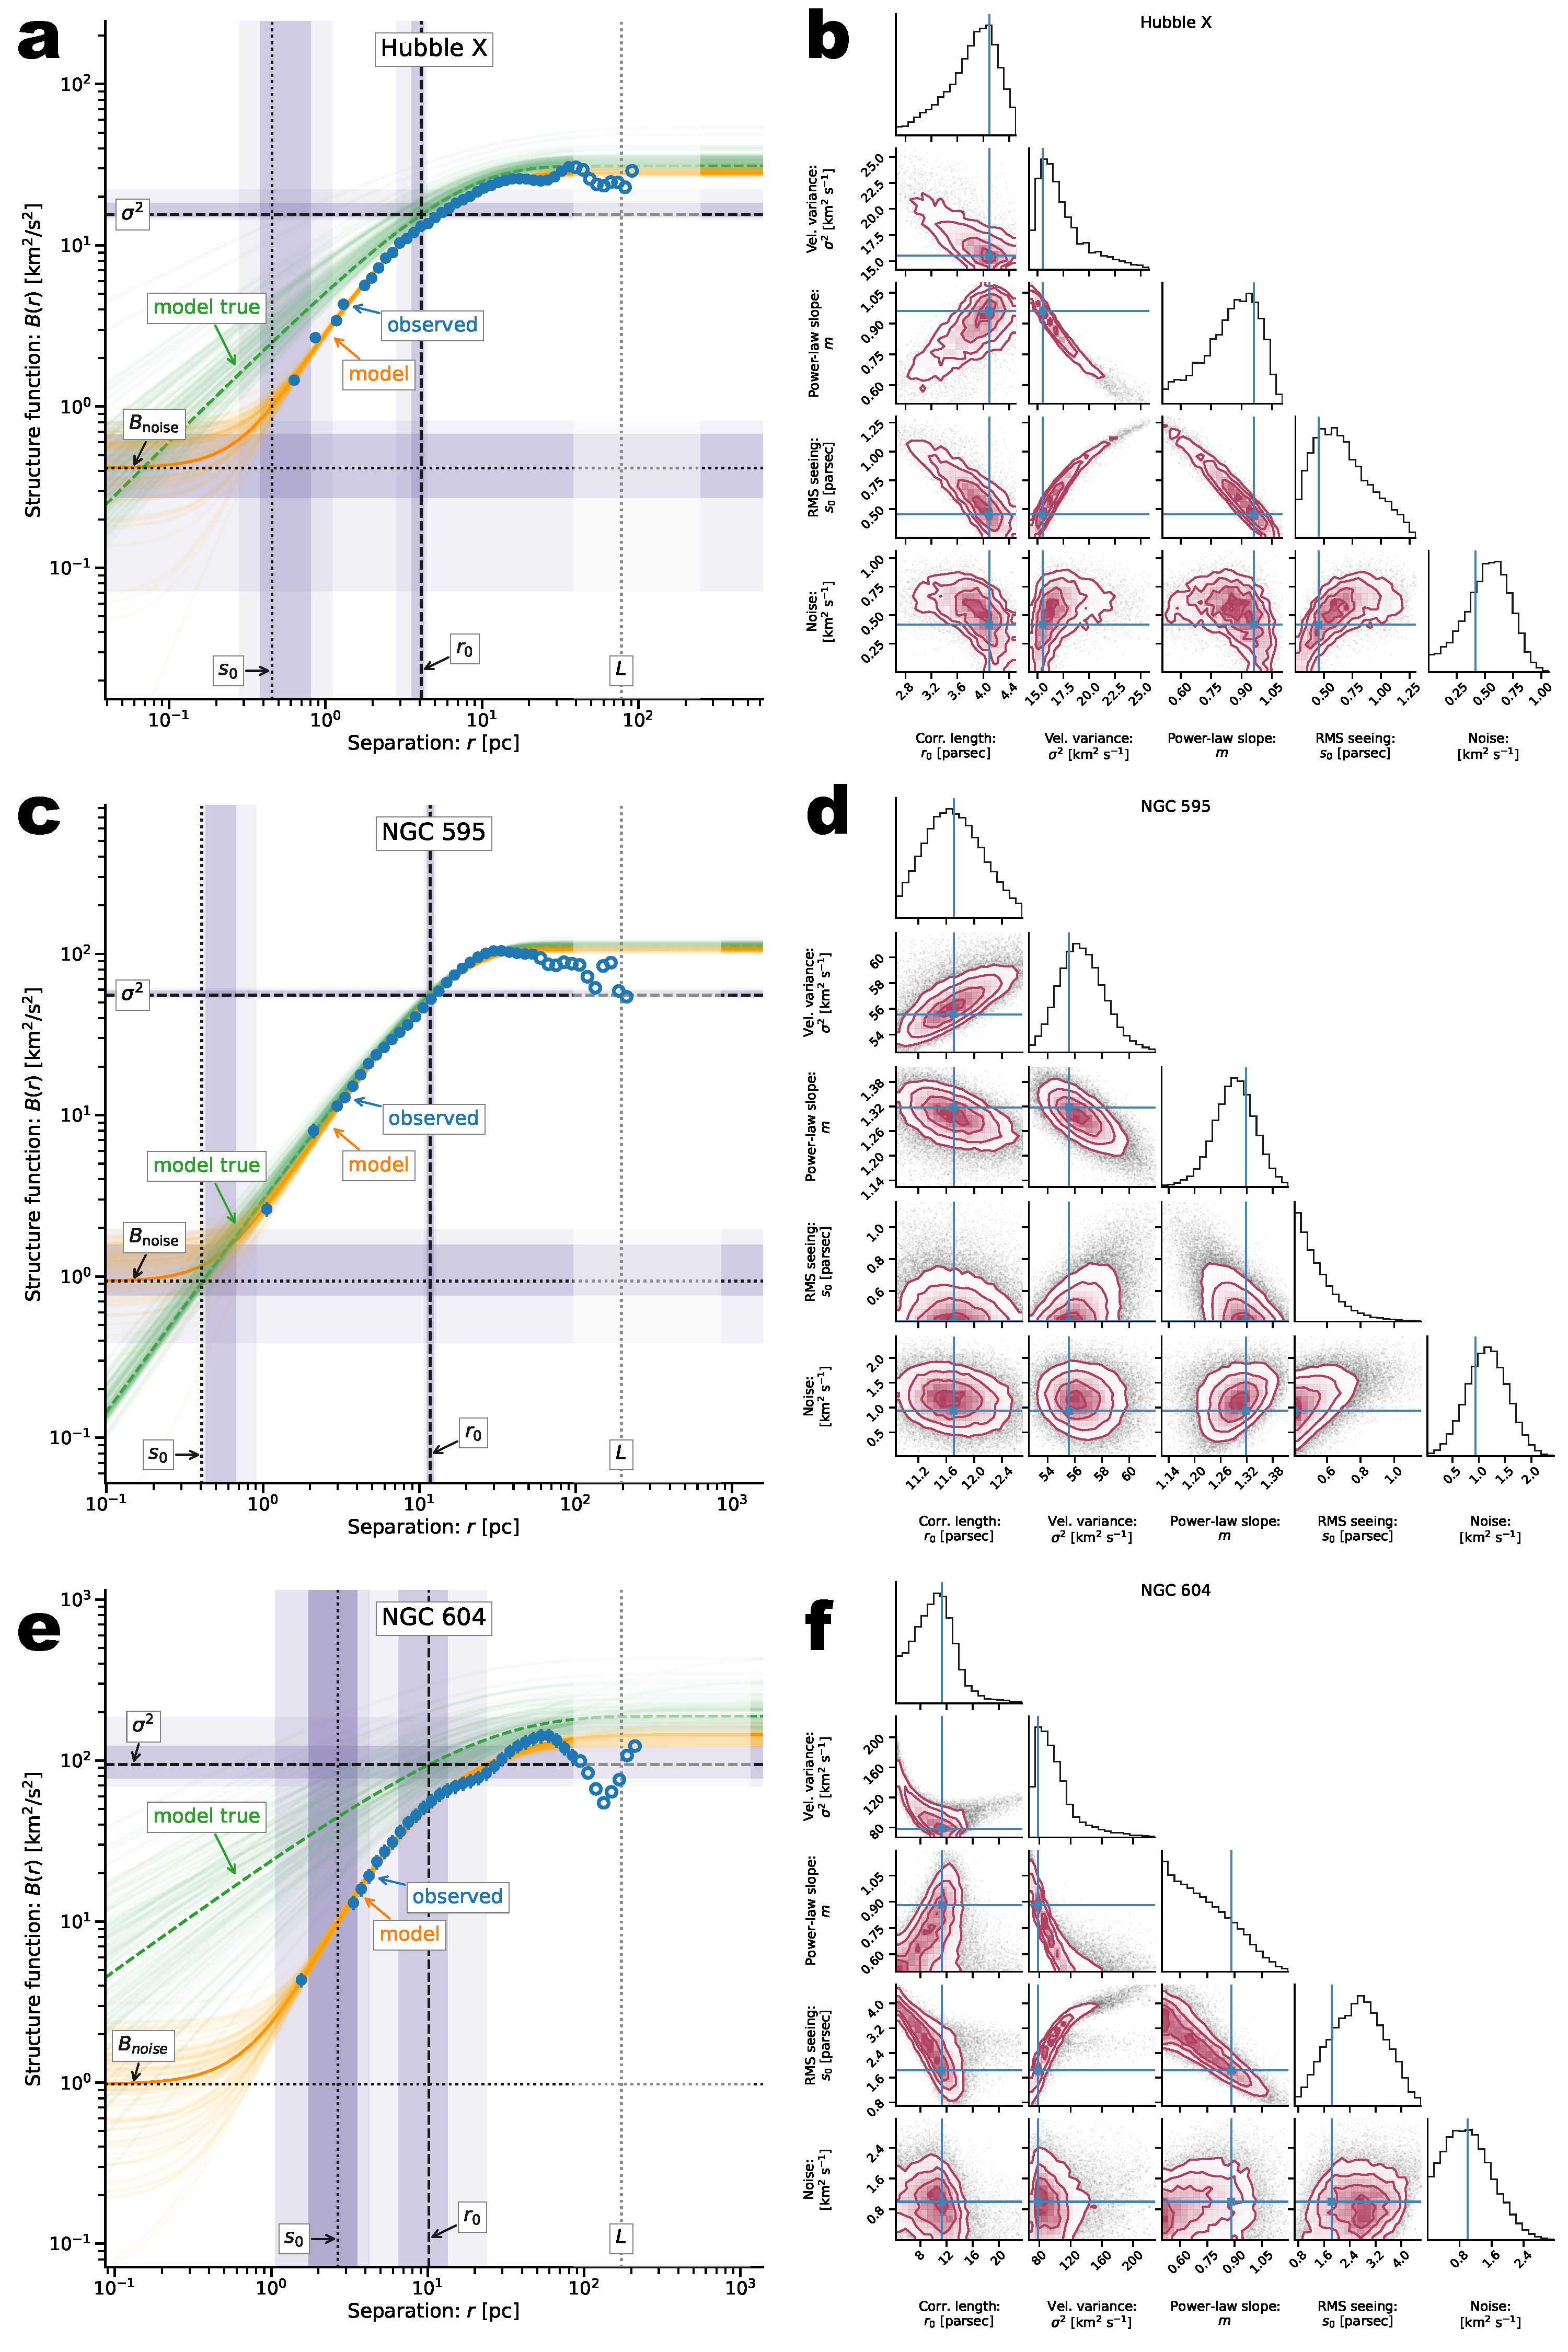
\includegraphics[width=0.8\linewidth]{Figures/strucfunc-fit-C}
  \caption{Second-order structure functions for the velocity centroid images of the \(H\alpha\) emission line}\label{fig:strucfunc-fit-C}
\end{figure*}

\begin{table*}
\begin{center}
\caption{Main results.}
\begin{tabular}{l CCCCCC}
\toprule
  Region &  \sigma^2\pos\quad [\si{km^2.s^{-2}}] 
         & B_{\text{noise}} \quad  [\si{km^2.s^{-2}}]  
         &  s0 \quad [\si{pc}] 
         &  r_0 \quad  [\si{pc}]
         &  L \quad [\si{pc}]
         & m  \\
\midrule
30 Dor &         300 \pm 9  &            6   \pm 1    &  0.16 \pm 0.02   &   4  \pm 0.2    &  32  &  0.84 \pm 0.04 \\
NGC 604 &         81 \pm 25 &            0.4 \pm 0.3  &   2.2 \pm 1.1    &   9  \pm 3.0    &  173 &  0.82 \pm 0.20 \\
NGC 595 &         56 \pm 2  &            1.2 \pm 0.4  &   0.5 \pm 0.1    &   12 \pm 1      &  196 &  1.3  \pm 0.05 \\
NGC 346 &         37 \pm 1  &            1.3 \pm 0.3  &  0.07 \pm 0.01   &   2  \pm 0.1    &  20  &  0.76 \pm 0.02 \\
Carina &          18 \pm 1  &              2 \pm 1    &  0.008 \pm 0.005 &  0.56\pm 0.04   &  20  &  1.14 \pm 0.10 \\
Hubble X &        16 \pm 2  &            0.5 \pm 0.2  &   0.6  \pm 0.3   &   4  \pm 0.4    &  78  &  0.88 \pm 0.14 \\
 Orion core &     13 \pm 1  &          0.025 \pm 0.002 & 0.002 \pm 0.0   &   0.07 \pm 0.01 &  0.5 &  1.07 \pm 0.02 \\
Hubble V &        10 \pm 1  &            0.1 \pm 0.1  &  0.5   \pm 0.1   &   3.4 \pm 0.3   &  61  &  0.74 \pm 0.1 \\
Lagoon &           7 \pm 1  &            0.2 \pm 0.1  &  0.005 \pm 0.003 &   1 \pm 0.2     &  16  &  1.13 \pm 0.1 \\
EON &              5 \pm 1  &              6 \pm 0.5  &  0.1   \pm 0.05  &   0.4 \pm 0.1   &  3   &  1.44 \pm 0.4 \\
\bottomrule
\end{tabular}\label{tab:Res}
\end{center}
\end{table*}

%%% Local Variables:
%%% mode: latex
%%% TeX-master: "strucfunc_paper"
%%% End:

%\begin{table*}
% \begin{center}\caption{Main results.
%  a) \citet{tanco1997}
%      b) \citet{2019arXiv191203543M}
%      c) \citet{Castro:2018a}
%      d) \citet{Damiani:2016a}
%      e) \citet{Damiani:2017b}
%      f) \citet{1987A&A...176..347H}
%      g) \citet{arthur2016turbulence}.}
% \begin{tabular}{ccccccccc}\hline
% HII         &\(\sigma^{2}\) &\(r_0\)                     &\(m\)    &\(\langle \sigma_{LOS} \rangle \) & Previously\\
% Region      &[km/s]$^{2}$     &[pc]                        &                           &  [km/s]& used in:\\ \hline
% NGC 604     & 80.93$\pm$25.31 &  9.12$\pm$2.98  & 0.82$\pm$0.20  & 16.2 & a,b \\
% NGC 595     & 56.45$\pm$1.69  & 11.69$\pm$0.45  & 1.29$\pm$0.04  & 18.3 & - \\
% Hubble X    & 15.55$\pm$1.50  &  3.90$\pm$0.28  & 0.94$\pm$0.12  & 13.4 & - \\ 
% Hubble V    & 10.46$\pm$0.75  &  3.42$\pm$0.33  & 0.73$\pm$0.09  & 12.3 & - \\  
% 30 Dor      & 350.87$\pm$21.59 & 4.60$\pm$0.43  & 0.84$\pm$0.03  & 31.7 & c\\
% Carina      & 16.74$\pm$1.13  & 0.66$\pm$0.08  & 1.36$\pm$0.29  & 22.4 & d\\
% NGC 346     & 38.03$\pm$1.09  & 1.90$\pm$0.09  & 0.78$\pm$0.02  & 10.2 & -\\
% Lagoon      & 7.29$\pm$0.84   & 1.00$\pm$0.17  & 1.12$\pm$0.09  & 13.6 & e\\ 
% Orion Large & 5.97$\pm$0.58   & 0.73$\pm$0.17  & 1.72$\pm$0.524 & 6.0 & f \\
% Orion Small & 16.92$\pm$0.97  & 0.091$\pm$0.006 & 1.06$\pm$0.01 & 6.0 & g \\\hline	  
% \end{tabular}\label{tab:Res}
% \end{center}
%\end{table*}  

\subsubsection{Velocity field \(\sigma\)}

The true variance of the velocity fields obtained with the analysis in Section \ref{sec:apply} is shown in the second column in Table \ref{tab:Res}. 
For all regions except for Carina and Lagoon there is an slight increase in the value of $\sigma$.

%The highest \(\sigma\) is 15.8 km s\(^{-1}\) for 30Dor.
%This is two times higher than NGC 604 that has a value of 7.4 km s\(^{-1}\), followed by NGC 595 with 6.64 km s\(^{-1}\).
%NGC 346 is next with a value of 5.6 km s\(^{-1}\), followed by Carina with 4.22 km s\(^{-1}\).
%Hubble X and M42 have a value of 3.59 and 3.23 km s\(^{-1}\), respectively.
%Hubble V has 2.8 km s\(^{-1}\) and last mof all sample is Lagoon with 2.7 km s\(^{-1}\).

\subsubsection{Structure function power indices \(m\)}

%As a justification for the use of the structure function we can consider that any relation between the line width and line-of-sight depth can be interpreted in terms of a correlation between velocity spread and scale size.
%This follows if we have an optically thin spectral line where it will have a width which is related to the total radial velocity dispersion of all fluctuations sampled along the line-of-sight \citep{1984ApJ...277..556S}. 
%In these sense the structure function is used as a tool to investigate the projection of a three-dimensional correlation function onto the plane of sky \citep{arthur2016turbulence}.

It has been proposed for comparison between two-dimensional observations and the three-dimensional value of the astronomical object what it is called projection smoothing \citep{von1951methode, munch1958internal,1987ApJ...317..686O}, where:

\begin{equation}\label{eq:exp1}
m_{2D}= m_{3D} + 1
\end{equation}

or when the astronomical object is almost two-dimensional (sheet-like) we have:

\begin{equation}\label{eq:exp2}
m_{2D} \sim m_{3D}
\end{equation}

If the extension of the region is compared with its depth the value of the index is $\frac{5}{3}$. While the case where the extension is much greater than its depth (two-dimensional) will have a value of $\frac{2}{3}$.

We can compute the $m_{3D}$ index from the two dimensional \(m\), if we assume that the $m_{3D}$ index lies between the limits of projection smoothing and a sheet-like distribution. 
Following the procedure by \cite{arthur2016turbulence} and assuming the relationship m$_{2D}$ - 1 $<$ m$_{3D}$ $<$ m$_{2D}$ we have 0.36 $<$ m$_{3D}$ $<$ 0.72.


\subsubsection{Significance on the length scale \(r_0\)}

Ideally the correlation length \(r_0\), should represent the scale of dominant energy injection. 
Since it is unclear what are the mechanisms driving the turbulence, thought a lot of options are candidates, it is difficult to pinpoint one particular process as the main responsible. 
The range covered in our results goes from 0.09 to 11 pc.

%%%%%%%%%%%%%%%%%%%%%%%%%%%%%%%%%%%%%%%%%%%%%%%%%%%%%%%%%%%%%%%%%%%%%%%%%%%%%%%%%%%%%%

\section{Discussion}\label{sec:discussion}

\subsection{Correlations between physical properties and turbulent parameters}

Relationship between the physical properties of HII regions, like size and luminosity, and the velocity dispersion have been used as tools for concluding scaling relations for these objects.
These relations have also been studied in dwarf galaxies and high-redshift star formation regions.
\citet{melnick1977,terlevich1981} were the first to shown an empirical relationship between the line width and the integrated properties of the HII regions as the diameter or the luminosity ($r \sim \sigma ^{\sim 2}$ ; $\text{L}_{\text{H}} \sim \sigma ^{\sim 4}$).
They conclude that GEHRs follow this relation because they behave as self-gravitatory systems like globular clusters or elliptical galaxies.
The work of \citet{1988A&A...201..199A} confirmed these relationships considering the discrepancies of previous investigations obtaining \(\text{L}_{\text{H}_{\alpha}} \propto \sigma^{3.9}\) and \(r \propto \sigma^{1.84}\).
%\citet{1981MNRAS.194..809L}



\citet{2012MNRAS.422.3339W} have found that clumps and HII regions follow scaling relations over the range of z = 0-2 for \halpha\ size, velocity dispersion, luminosity and mass, finding \(\sigma \propto r^{0.42}\), \(\text{L}_{\text{H}_{\alpha}} \propto r^{2.72}\) and \(\text{L}_{\text{H}_{\alpha}} \propto \sigma^{4.18}\), respectively. 
This results imply that the same process are seen at high redshifts and the current epoch in star forming regions.
Recently, \citet{Moiseev:2015a} found that the relation in dwarf galaxies is \(\text{L}_{\text{H}_{\alpha}} \propto \sigma^{5}\).
\citet{2018MNRAS.474.1250F} presented the relationship between integrated H$_{\beta}$ line luminosity and the velocity dispersion for new data of 36 giant HII regions obtaining \(\text{L}_{\text{H}_{\beta}} \propto \sigma^{5.02 \pm 0.21}\).

This line of investigation is followed using the scaling relation as a research tool between the properties of the sample of HII regions and our results. 
We use the properties in Table \ref{tab:Reg} with the turbulent parameters in Table \ref{tab:Res} as the dependent variable to adjust a fit in the form $Y = aX +b$. 
For this procedure we use a hierarchical Bayesian approach using the package \textit{linmix} \citep{2007ApJ...665.1489K}.
The results are shown in Table \ref{tab:RestStats} in ascending order for the p-value.
In the Figures \ref{fig:rvsR}-\ref{fig:svss} we show the correlations with a significance level  $p \leq $0.10.
In all the figures the slope of the fit shown in solid black line is the mean of all red lines that reflect the posterior of the Bayessian analysis.

The Figure \ref{fig:rvsR} shows the strongest correlation, being this between the correlation length $r_0$ and the size $R$ of the region. The relationship we found is relation of $\log r_0 = (0.69 \pm 0.07) \log R-(0.85 \pm 0.14)$.

The Figure \ref{fig:sigvsl} shows the log $\sigma$-log $\text{L}(\text{H}_{\alpha})$ plane.
Since this relation is the most common it can be use for comparison with the investigations mentioned at the beginning of this section.
Our results give us a relation of $\log \sigma = (0.16 \pm 0.12) \log \text{L}(\text{H}_{\alpha})-(5.6 \pm 5.0)$.
It is customary in the literature to present $\text{L} (\text{H}_{\alpha})$ as the dependent variable.
In our case if we choose the upper positive error and take the inverse of slope we have \(\text{L}_{\text{H}_{\alpha}} \propto \sigma^{3.5}\). 
Using the same procedure in \textit{linmix} and changing the variables we obtained $\log \text{L}(\text{H}_{\alpha}) = (3.32\pm 1.89) \log \sigma -(36.23 \pm 1.45)$.
Both relations are close to the previously proposed \(\text{L}_{\text{H}_{\alpha}} \propto \sigma^{4}\)


\begin{table*}
\begin{center}
\caption{Linear regressions values in the form Y = aX + b between our turbulent parameters obtained using the chi-square statistic and properties of each region (Table \ref{tab:regions-properties}). The fifth column, $r$, is the Pearson correlation coefficient and the last column is the $p$-value. This results were obtained using the procedure in \citet{2007ApJ...665.1489K}.}
\begin{tabular}{RRRRRR}
  \toprule
  Y &                   X &                 a &                 b &       r &      p \\
  \midrule
  \log r_0 &         \log D_{\hii} &   0.95 \pm 0.33 &  -1.68 \pm 0.71 &   0.86 &  \mathbf{0.003} \\
  \log \sigma\pos &        \log L(\ha) &    0.25 \pm 0.11 &  -9.01 \pm 4.26 &   0.81 &  \mathbf{0.008} \\
  \sigma\los &  \sigma\pos &   1.03 \pm 0.45 &   7.40 \pm 2.88 &   0.78 &   \mathbf{0.010} \\[\smallskipamount]
  \log \sigma\pos &         \log D_{\hii} &   0.26 \pm 0.18 &   0.20 \pm 0.39 &   0.64 &   0.06 \\
  \log \sigma\pos &   \log r_{0} &    0.19 \pm 0.18 &   0.68 \pm 0.13 &   0.51 &  0.16 \\
  \log m &  \log d &  -0.02 \pm 0.04 &   0.04 \pm 0.08 &   -0.40 &   0.29 \\
  \log m &  \log  \sigma\pos &  -0.11 \pm 0.20 &   0.09 \pm 0.16 &  -0.37 &  0.33 \\
  \log m &  \log  r_{0} &   -0.02 \pm 0.07 &   0.02 \pm  0.05 &  -0.28 &  0.47 \\
  \bottomrule
\end{tabular}\label{tab:RestStats}
\end{center}
\end{table*}


%<10\(^{-5}\)

%%% Local Variables:
%%% mode: latex
%%% TeX-master: strucfunc_paper
%%% End:


\begin{figure}
\centering 
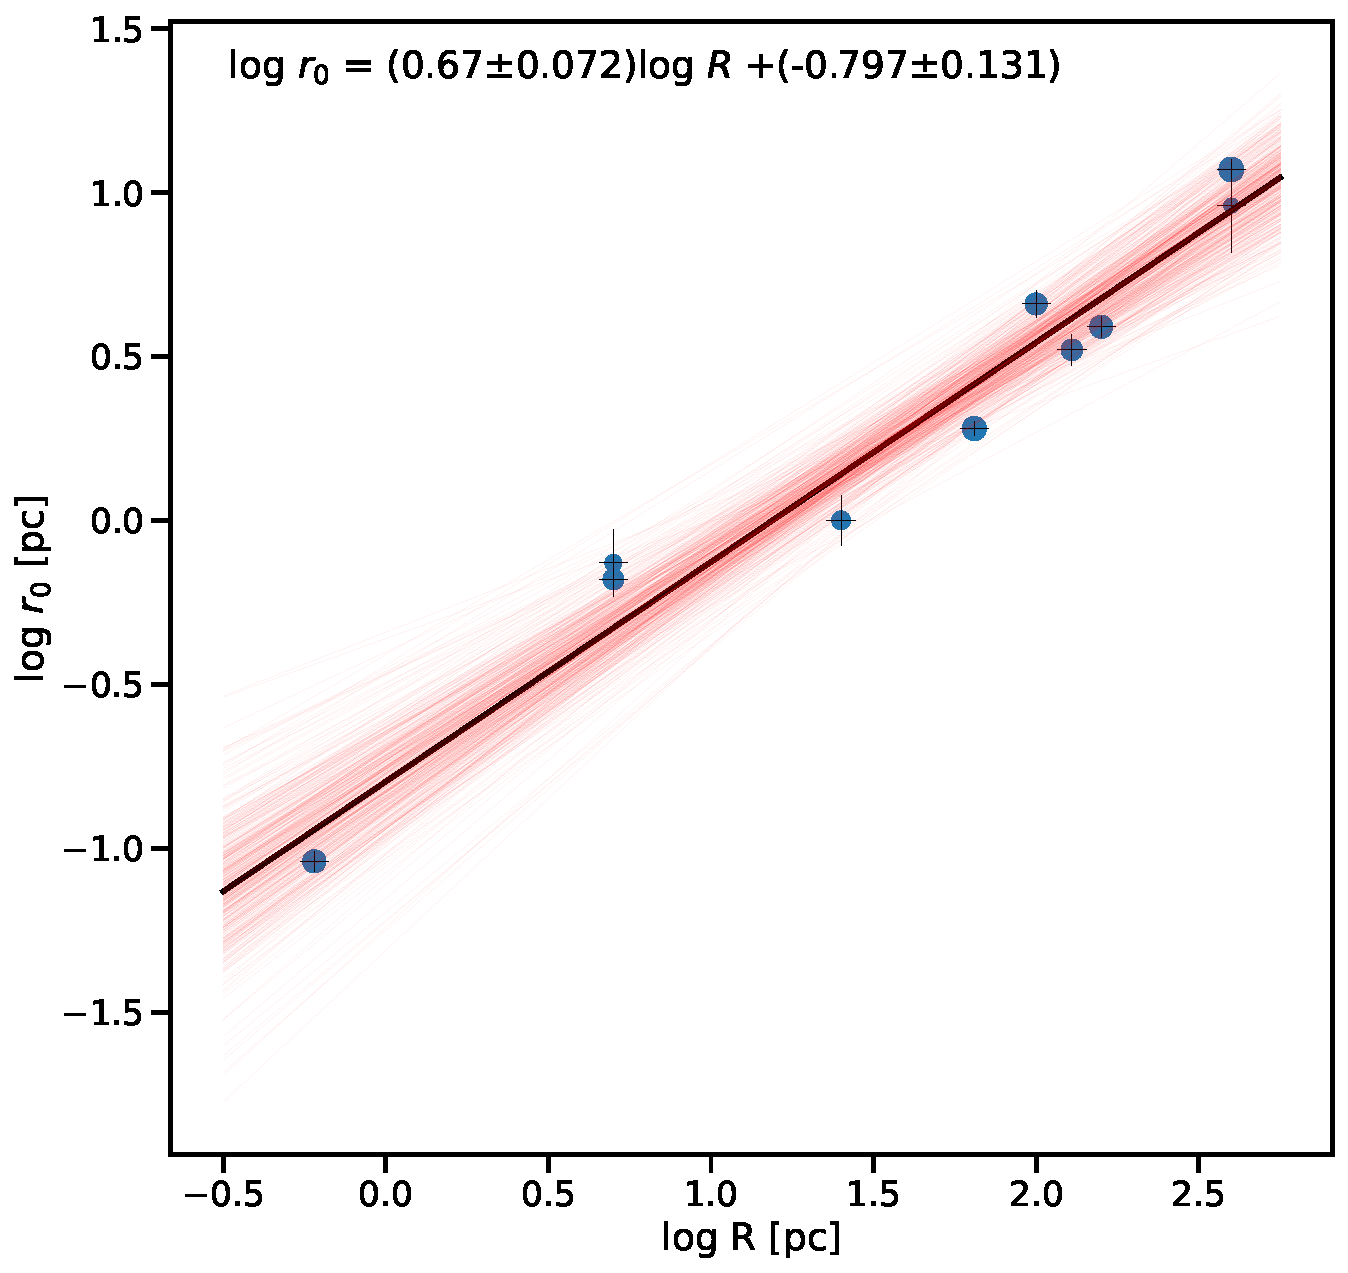
\includegraphics[width=3in]{Figures/rvsR}
\caption{The log $r_0$-log $R$ plane derived form our results an data in the literature. A fit with slope of 0.67$\pm$0.07 is shown in solid black line that is the mean of all red lines that reflect the posterior of the Bayessian analysis. }
\label{fig:rvsR}
\end{figure}

\begin{figure}
\centering 
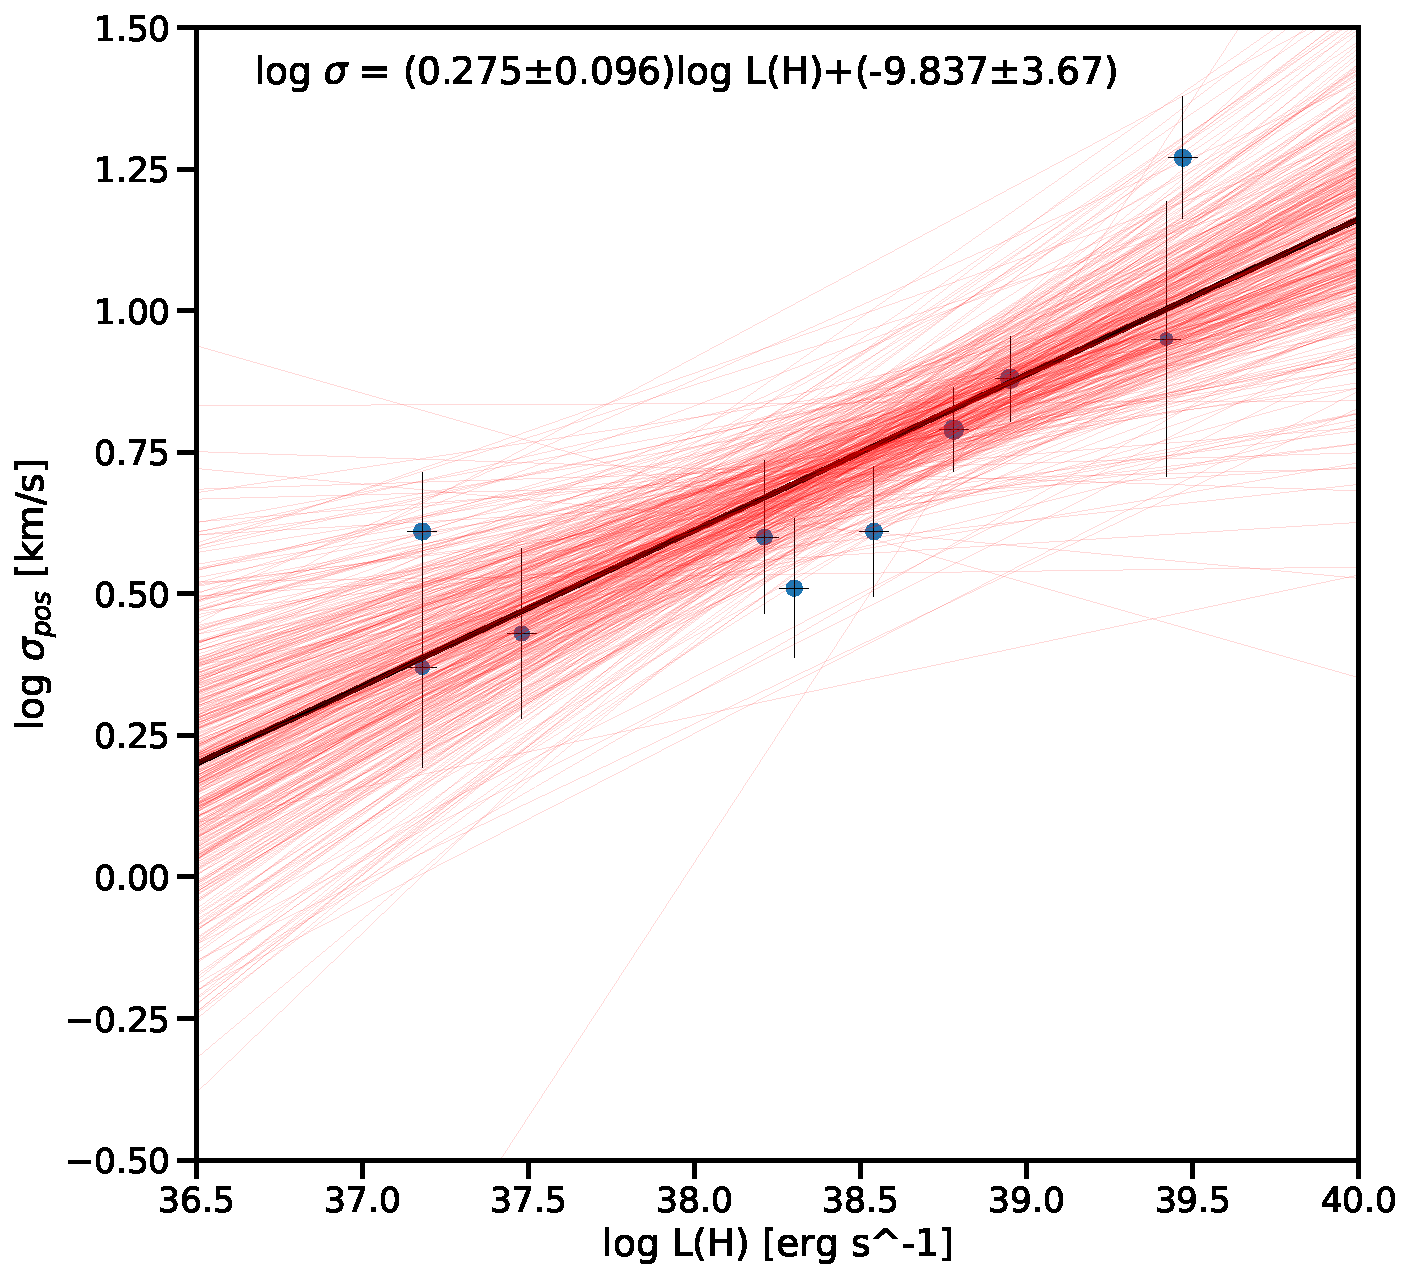
\includegraphics[width=3in]{Figures/svsL}
\caption{Same as Fig. \ref{fig:rvsR} but for the log $\sigma$-log $L(H_{\alpha})$ plane.}
\label{fig:sigvsl}
\end{figure}

\begin{figure}
\centering 
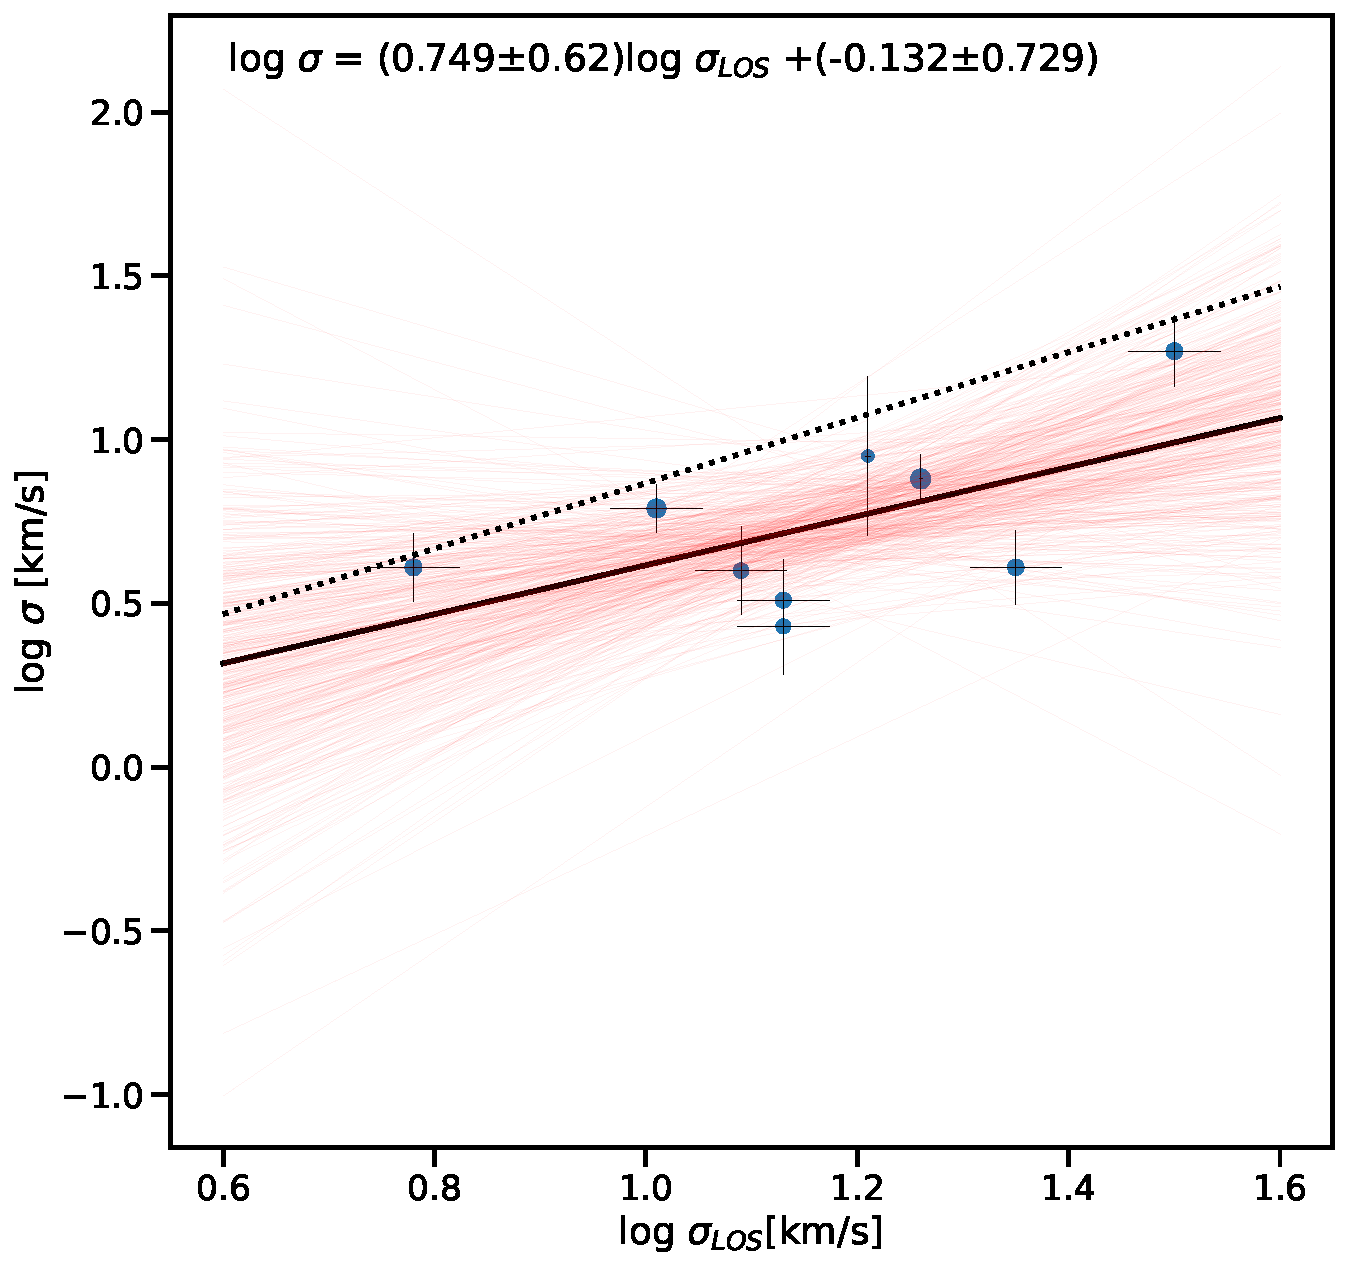
\includegraphics[width=3in]{Figures/svss.pdf}
\caption{Same as Fig. \ref{fig:rvsR} but for the log $\sigma$-log $\sigma_{\text{LOS}}$ plane. The dotted line represents slope equal to unity.}
\label{fig:svss}
\end{figure}

\subsubsection{Relationship between plane-of-sky and line-of-sight velocity dispersion.}

The broad in the velocity width of the emission line represents the range of velocities along the line-of-sight (LOS), among thermal movements. 
We can consider as a main broadening mechanisms, the kinematical disorder along the LOS related to velocity gradients by the clumpiness on the molecular cloud and turbulent movements.
On the plane-of-sky (POS) the consequences of those gradients and movements is measured in every pixel. The spatial variations on the velocity field would depend on the targeted pixel, depending on the motions inside the cloud (the LOS component).
This reasoning has lead to \citet{2011MNRAS.413..705L} to propose a direct relationship between \(\sigma_{\text{LOS}}\) and \(\sigma_{\text{POS}}\) (or just \(\sigma\) in this work).

It have been mentioned that the projection of the velocity fluctuations reduces the actual amplitude in the line-of-sight \citep{1984ApJ...277..556S,arthur2016turbulence}.
We can see from Table \ref{tab:Res} that the line-of-sight velocity dispersion is roughly twice the plane-of-sky velocity dispersion.
In the case of homogeneous turbulent velocity we can consider the effect of \textit{project smearing} \citep{1984ApJ...277..556S}, where the projection from three to two dimensions over the line-of-sight depth \(H\), reduces the plane-of-sky amplitude for the condition \(r_{0} < H\).
With a value of \(\sigma / \sigma_{\text{LOS}}\) = 0.5 we obtain \(r_{0} / H \sim\) 0.01-0.1.

The Figure \ref{fig:svss} shows the log $\sigma$-log $\sigma_{\text{LOS}}$ plane with a relationship of $\log \sigma = (0.75 \pm 0.60) \log \sigma_{\text{LOS}}-(0.13 \pm 0.70)$ .

\subsection{Comparison with previous structure functions}

In Section \ref{sec:apply} we mentioned the reduced chi-square method we are using for determining the correlation length and the index of the slope. Since this is the first time this method is applied to a sample of HII regions (at least for our knowledge), the results are bounded to be different from previous investigations, including the one that have the same observations as \citet{arthur2016turbulence} and \citet{2019arXiv191203543M}. 

A complete analysis on different emissions lines of the structure function on Orion was carried out by \citet{arthur2016turbulence} and reference therein. 
They observed a tendency that higher ionization lines presents higher values on the magnitude dispersion and the steepness of the structure function slope. 
This results just consider one component on the Gaussian fit. 
The power-law index obtained by \citet{arthur2016turbulence} are \(m \sim 1.2 \pm 0.1\) for \halpha\ and [OIII] emission lines and for [SII] they found \(m \sim 0.8 \pm 0.1\). 
The correlation length for all lines is \(\approx\) 0.05 pc. For the same \halpha\ observation we obtained a value of 1.06$\pm$0.01 and a correlation length of 0.092$\pm$0.007 pc. 

The first attempt at characterizing turbulence in a giant extragalactic HII region, GEHR, was done by \citet{1961MNRAS.122....1F} with the 30 Doradus complex in the LMC, finding no indication of turbulent motions between scale of 10 and 100 pc.
\citet{2019arXiv191203543M} also investigated the structure function in 30 Doradus finding on their results that the structure function is entirely flat on scales from 3 to 200 pc.
In the context of the high-resolution observations it is possible to see why their results do not reflect the turbulent structure of the nebula; their observations cover a region where the large-scale velocity fluctuations are uncorrelated.
There is a good agreement with the single-Gaussian fit results from \citet{2019arXiv191203543M} (Figure 15 Top on their work), while \citet{1961MNRAS.122....1F} results do not overlap with ours.
From this analysis this is the first time turbulence characterized in 30 Doradus using the structure function.

There is broad agreement in our structure function results and previous studies that consider NGC 604, mainly because where are using the same data \citep{Medina-Tanco:1997a, Melnick:2021x}. 
from \citet{Medina-Tanco:1997a} and \citet{Melnick:2021x}, and using the same TAURUS-II data.
Despite this general agreement the interpretations in each study is different.
\citet{Medina-Tanco:1997a} conclude about a double regime acting on the kinetic energy spectrum.
According to this double cascading, turbulence is being forced at scales of \(\approx\)10 pc while and energy cascade has developed down to the smallest scales and other, as an inverse cascade, extends up to scale of \(\approx\)70 pc.
Interesting enough, \citet{Medina-Tanco:1997a} mentioned various characteristic scale lengths, the most notorious is the \(\approx\)10 pc, a value close to our correlation length of \(\approx\)9 pc, and they interpret it as possible source on energy associated with the expansion of shocks coming from wind bubbles.  
None of the previous studies present a power-law index for the structure function to compare our results.
\citet{2019arXiv191203543M} addresses some issues with TAURUS II data while comparing profiles between the previous instrument TAURUS I where there exist a difference between observations (see section 4.1 on their paper).
As we agree with them in the importance of observing NGC 604 at higher spatial resolution, we have prove that a consistent method in analyzing structure function is key to obtaining trustworthy results.

For our NGC 595 \halpha\ emission line results there is no correspondence in the structure function between our results and previous investigations.
Our observations cover the brightest part of the region and have smaller resolution.
\citet{lagrois2009multi} and \citet{lagrois2011} structure functions results does not cover scales $<$10 pc, where in our results the correlation is taking place.
\citet{lagrois2011} used the data from \citet{lagrois2009multi} to complement the structure function analysis with the auto correlation function and filters to the velocity field to get rid of non-turbulent movements.
Their sigma is 5.92$\pm$0.15 km/s with a correlation length is 43 pc.
The power-law index they provide is 1.55$\pm$0.01.

%%%%%%%%%%%%%%%%%%%%%%%%%%%%%%%%%%%%%%%%%%%%%%%%%%%%%%%%%%%%%%%%%%%%%%%%%%%%%%%%%%%%%%%%%%%%%%%%%%%%%%%%%%%%%%%%%%%%%%

\section{Conclusions}\label{sec:conclusions}

The previous analysis was able to characterize the turbulence by determining a single inertial scale where the ionized gas behavior can be described by means of a power law.
To determine the inertial scale more precisely than in previous works, a new functional form was proposed for the second-order structure function that considers observational effects such as: seeing, noise and the size of the observational box.
These effects had not been considered in detail before and have important consequences is the interpretation of the inertial scale.

The new functional form of the structure function accurately determines the important parameters related to turbulence which are: the correlation length, the exponent of a power law that fits the results and the real variance of the region.
Compared to the majority of previous works, the previous parameters had been calculated using the criteria of each author.
A chi-square adjustment was performed using Bayesian statistics to determine the confidence intervals for each parameter.

This proposed analysis can be expanded to other HII regions with the possibility of comparing the results between them since the proposed method guarantees their homogeneity and the ability to develop a future catalog of these regions in a coherent way.
It could even be used to investigate the velocity fields of other phases of the interstellar medium.
The study of turbulence between ionized regions and the molecular clouds that give them birth can be carried out in a concise way, having the correct methods with the intention of advancing the understanding of the kinematic relationships between them.

\begin{enumerate}
\item For 30 Doradus with an observational box size of 32 pc an index of 0.84$\pm$0.03 is obtained with an inertial scale between 0.1 and 5 pc, and with a variance of 350$\pm$21 km$^2$/s$^2$. 
    
\item For NGC 604 with an observational box size of 173 pc an index of 0.82$\pm$0.20 is obtained with an inertial scale between 2 and 9 pc, and with a variance of 81$\pm$25 km$^2$/s$^2$.
    
\item For NGC 595 with an observational box size of 196 pc an index of 1.3$\pm$0.04 is obtained with an inertial scale between 0.5 and 12 pc, and with a variance of 56$\pm$1.6 km$^2$/s$^2$.

\item For NGC 346 with an observational box size of 20 pc an index of 0.78$\pm$0.02 is obtained with an inertial scale between 0.06 and 2 pc, and with a variance of 38$\pm$1.0 km$^2$/s$^2$.

\item For Orion with an observational box size of 0.45 pc an index of 1.06$\pm$0.02 is obtained with an inertial scale between 0.002 and 0.09 pc, and with a variance of 17$\pm$1.0 km$^2$/s$^2$.

\item For Carina with an observational box size of 20 pc an index of 1.36$\pm$0.30 is obtained with an inertial scale between 0.008 and 0.6 pc, and with a variance of 17$\pm$1.0 km$^2$/s$^2$.

\item For Hubble X with an observational box size of 78 pc an index of 0.94$\pm$0.12 is obtained with an inertial scale between 0.5 and 4 pc, and with a variance of 15.5$\pm$1.5 km$^2$/s$^2$.

\item For Hubble V with an observational box size of 61 pc an index of 0.72$\pm$0.09 is obtained with an inertial scale between 0.5 and 3 pc, and with a variance of 10.6$\pm$0.8 km$^2$/s$^2$.

\item For Lagoon with an observational box size of 16 pc an index of 1.12$\pm$0.09 is obtained with an inertial scale between 0.005 and 1 pc, and with a variance of 7.2$\pm$0.8 km$^2$/s$^2$.


    
\end{enumerate}

%%%%%%%%%%%%%%%%%%%%%%%%%%%%%%%%%%%%%%%%%%%%%%%%%%%%%%%%%%%%%%%%%%%%%%%%%%%%%%%%%%%%%%%%%%%%%%%%%%%%%%

\section*{Acknowledgements}

Based on observations made with KPNO telescopes
\textit{complete KPNO acknowledgment}.
Based on observations made with ESO Telescopes at the La Silla Paranal Observatory under programme IDs 076.C-0888 and 098.D-0211.
Based on observations made as part of the Gaia-ESO Spectroscopic Survey
\textit{complete Gaia-ESO acknowledgment}.
Based on observations made with the WHT
\textit{complete WHT acknowledgment}.
JGV acknowledges and thanks CONACyT-Mexico for a PhD research scholarship.
We are grateful to Norberto Castro Rodríguez for providing maps of emission line velocity moments for 30 Doradus derived from MUSE-VLT observations.

%%%%%%%%%%%%%%%%%%%%%%%%%%%%%%%%%%%%%%%%%%%%%%%%%%
%%%%%%%%%%%%%%%%%%%% REFERENCES %%%%%%%%%%%%%%%%%%

\bibliographystyle{mnras}
\bibliography{bibphd}

%\clearpage

%%%%%%%%%%%%%%%%%%%%%%%%%%%%%%%%%%%%%%%%%%%%%%%%%%
%%%%%%%%%%%%%%%%% APPENDICES %%%%%%%%%%%%%%%%%%%%%
%%%%%%%%%%%%%%%%%%%%%%%%%%%%%%%%%%%%%%%%%%%%%%%%%%

\appendix

\section{Degradation of the structure function due to observational limitations}
\label{sec:degr-struct-funct}
Studied in context of \(\Delta\)-variance by \citet{Bensch:2001l}.

\subsection{Finite box effects}
\label{sec:finite-box-effects}


\begin{figure}
  \begin{tabular}{@{} l @{}}
    (a)\\
    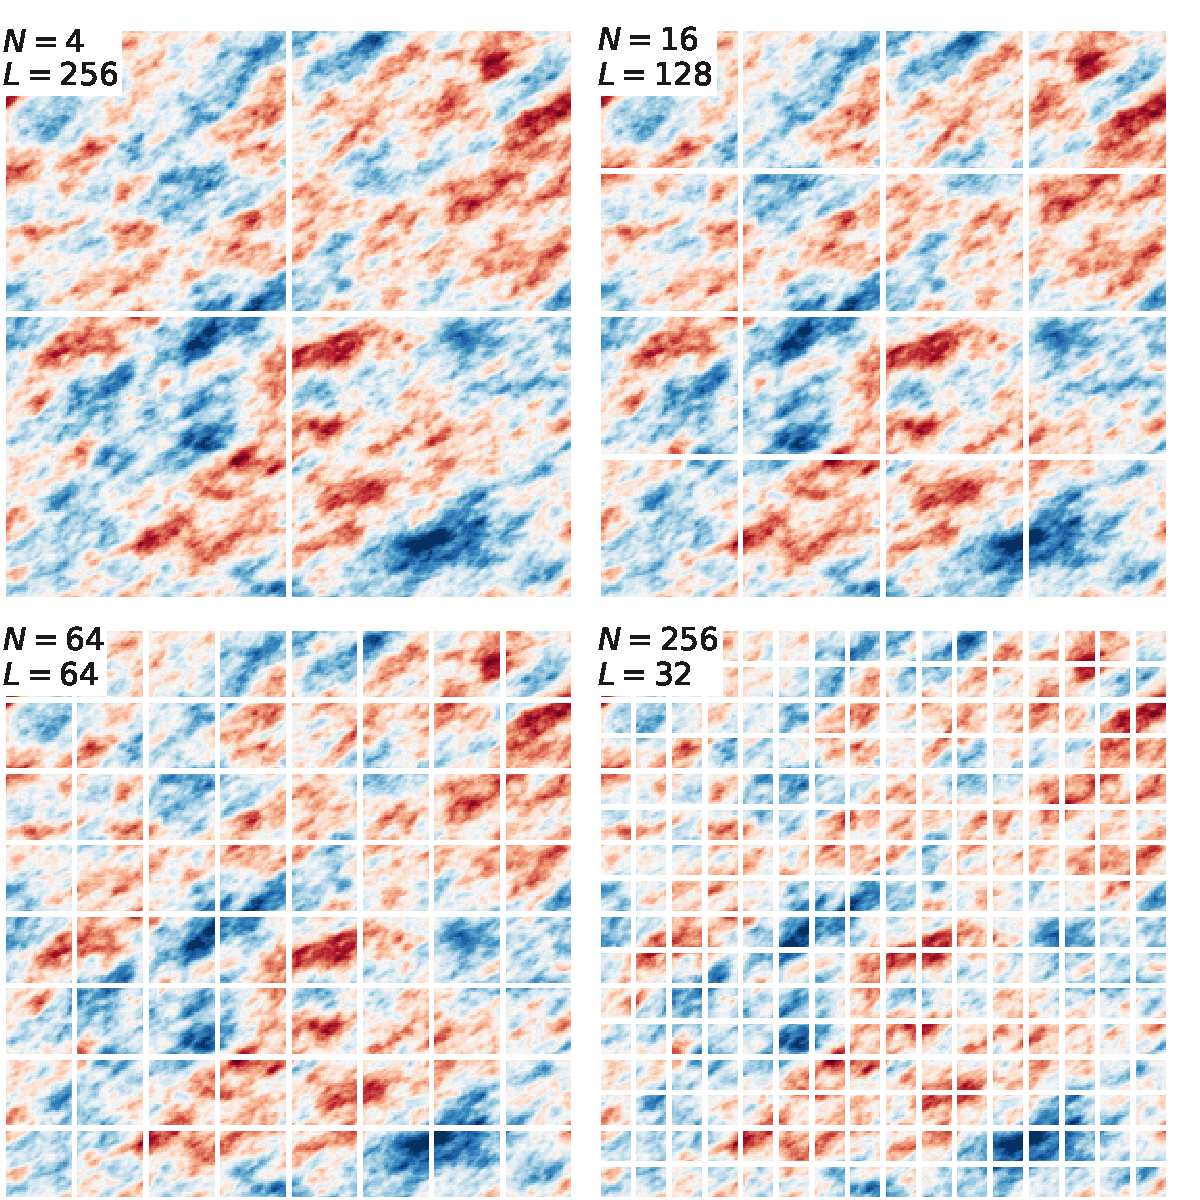
\includegraphics[width=\linewidth]{Figures/fake-finite-box-images}
    \\[\bigskipamount]
    (b)\\
    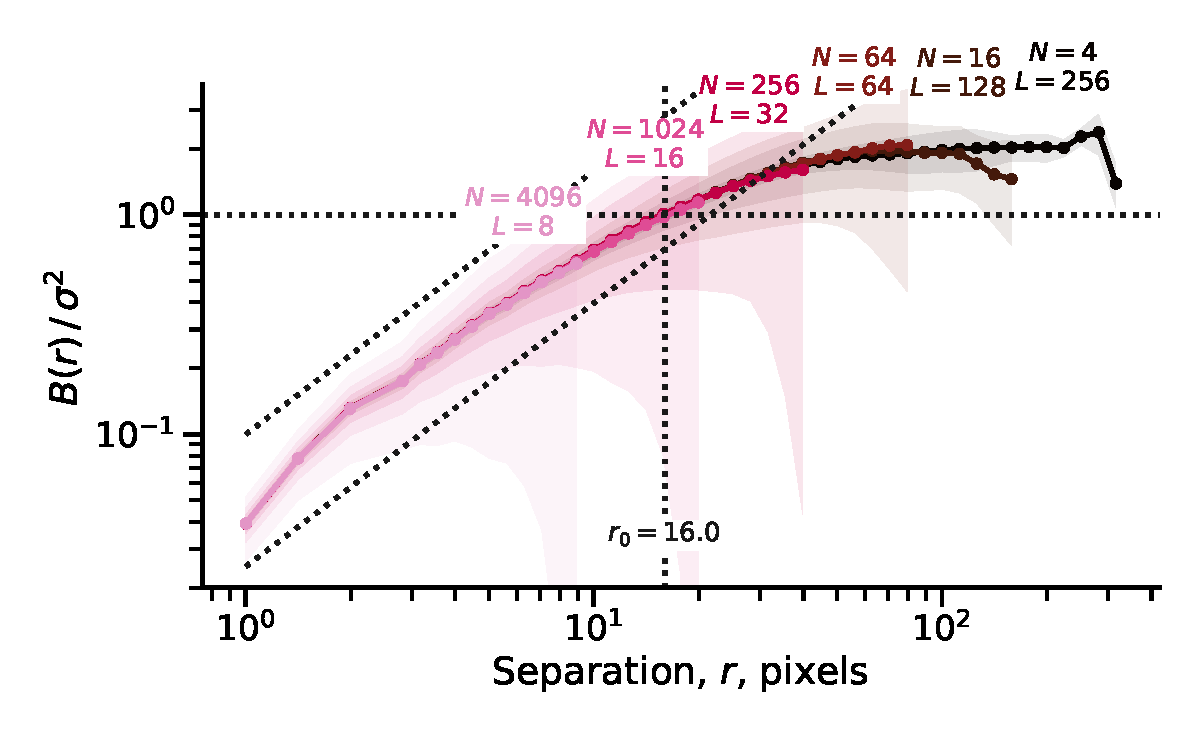
\includegraphics[width=\linewidth]{Figures/fake-finite-box-strucfunc}
  \end{tabular}
  \caption{Effects of finite box size on the structure function.
    (a)~Construction of simulated turbulent velocity fields of different sizes
    by repeated division of an initial field of size \(512 \times 512\) pixels.
    The \(j\)th level of division yields \(N = 4^j\) fields,
    each of linear size \(L \times L\) where \(L = 2^{9 - j}\). 
    (b)~Resultant structure functions.
  }
  \label{fig:finite-box}
\end{figure}

\begin{figure}
  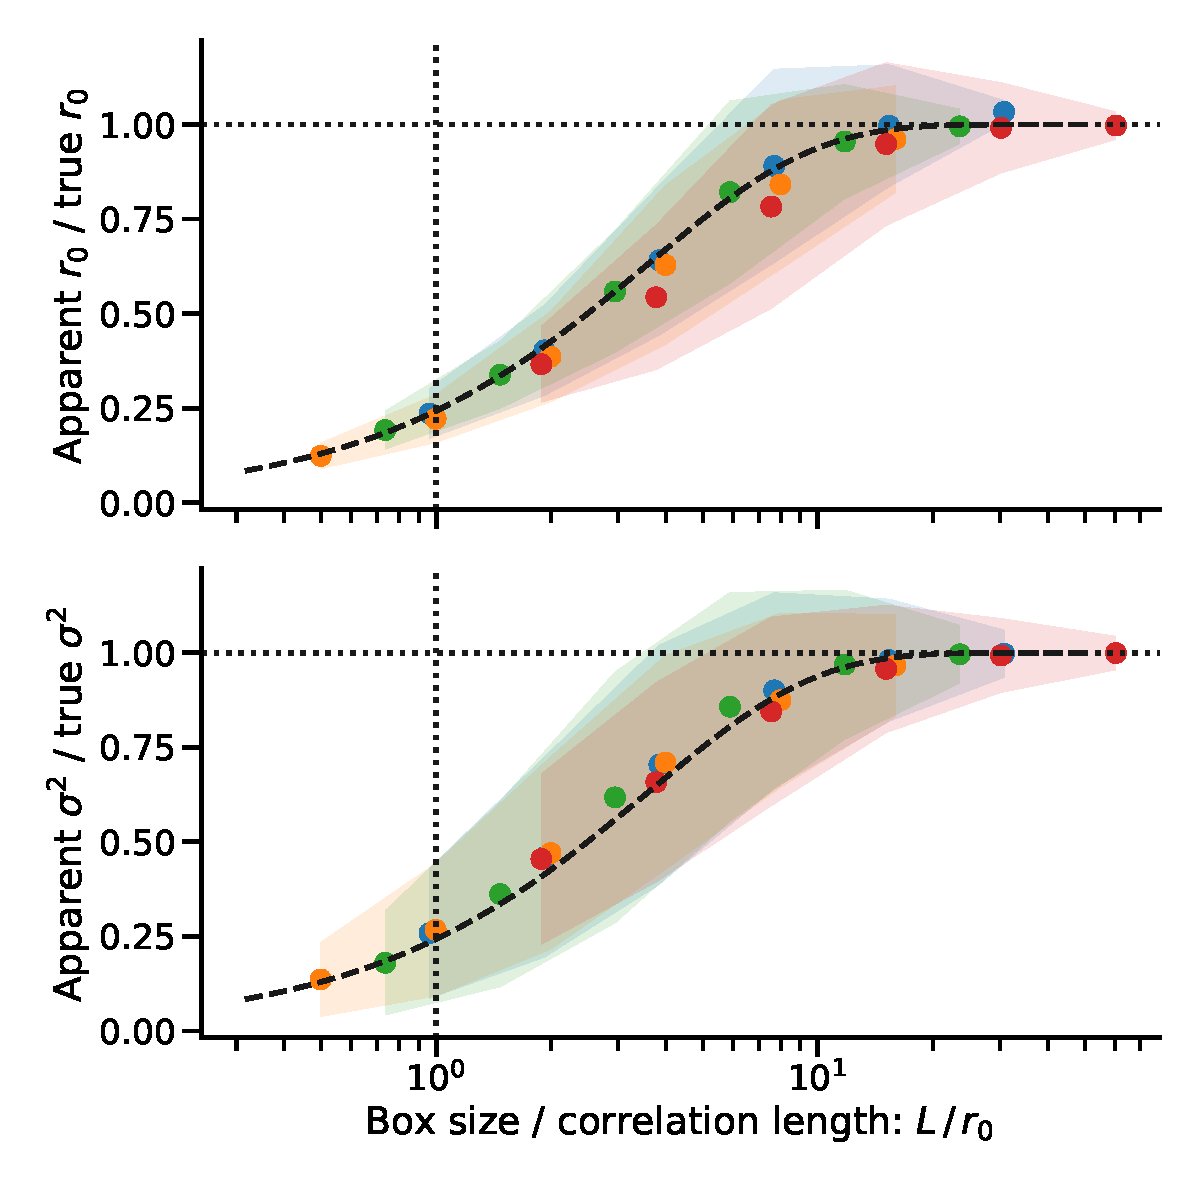
\includegraphics[width=\linewidth]{Figures/fake-finite-box-effect}
  \caption{
    Reduction of apparent velocity variance and correlation length
    due to finite box size.
  }
  \label{fig:finite-box-effect}
\end{figure}



\subsection{Effects of seeing}
\label{sec:effects-seeing-struc}


\begin{figure}
  \begin{tabular}{@{} l @{}}
    (a)\\
    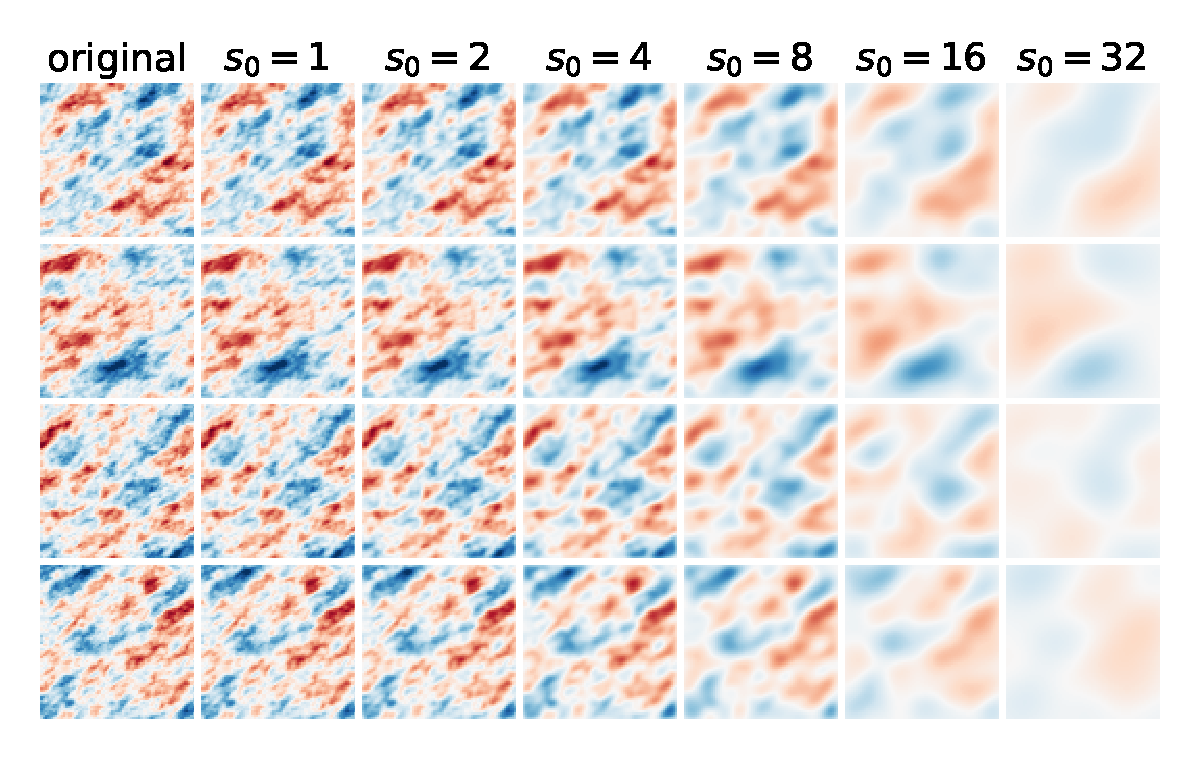
\includegraphics[width=\linewidth]{Figures/fake-seeing-nonp-thumbnails}\\
    (b)\\
    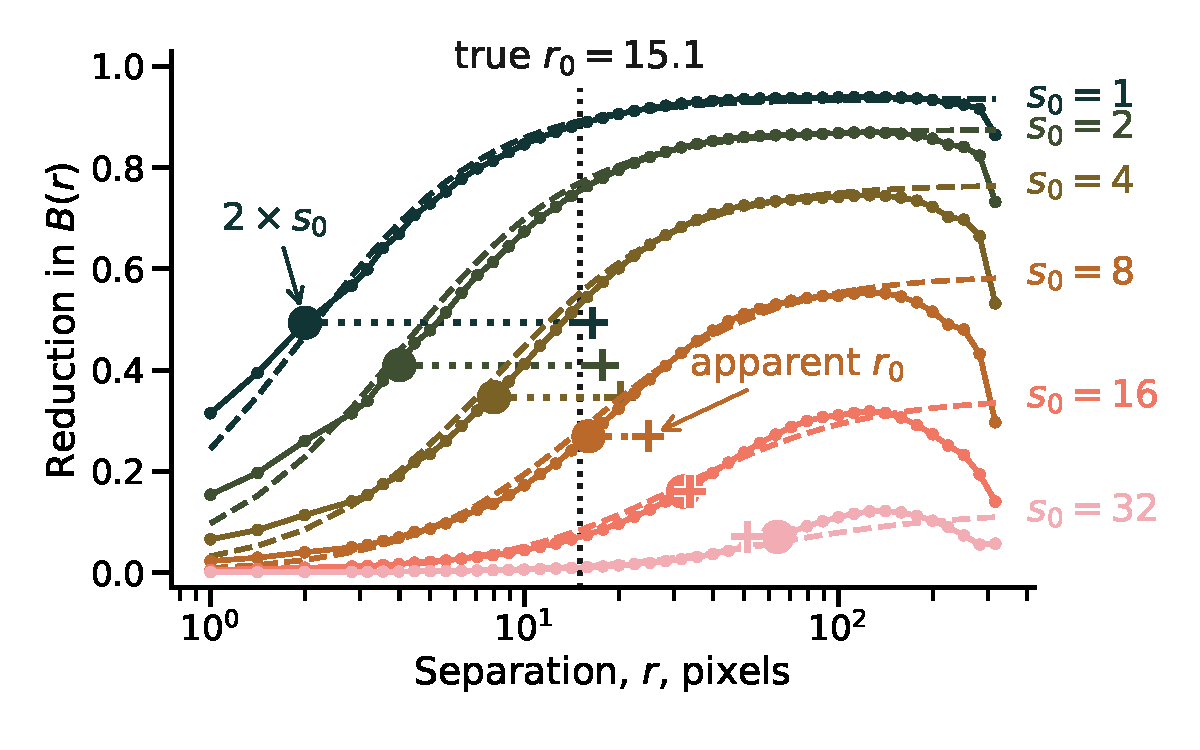
\includegraphics[width=\linewidth]{Figures/fake-seeing-nonp-reduction}
  \end{tabular}
  \caption{Effects of seeing on the structure function.
    (a)~Each row shows a different simulated random velocity field on a \(256^2\) grid
    (see text for details).
    The left column shows the original field,
    while the remaining columns show the effects of smoothing by a gaussian kernel
    with RMS width \(s_0\) from 1 to 32 pixels.
    The same color scale is used for all columns, ranging from \(-3\) to \(+3\) times
    the standard deviation of the unsmoothed map.
    (b)~Relative change in the second-order structure function due to the gaussian smoothing.
    Solid lines with symbols show the average over the 4 maps of
    \(B(r, s_0) / B(r, s_0 = 0)\) as a function of separation \(r\),
    with a separation of \(2 s_0\) indicated by a large filled circle on each curve.
    Dashed lines shows the empirical fit discussed in the text.
    The dotted line shows the correlation length of the original fields,
    while colored plus symbols show the apparent correlation length of the smoothed fields.
  }
  \label{fig:seeing-reduction}
\end{figure}


%%%%%%%%%%%%%%%%%%%%%%%%%%%%%%%%%%%%%%%%%%%%%%%%%%
%%%%%%%%%%%%%%%%%%%%% END %%%%%%%%%%%%%%%%%%%%%%%%
%%%%%%%%%%%%%%%%%%%%%%%%%%%%%%%%%%%%%%%%%%%%%%%%%%

% Don't change these lines
\bsp	% typesetting comment
\label{lastpage}
\end{document}

% End of mnras_template.tex
%%% Local Variables:
%%% mode: latex
%%% TeX-master: t
%%% End:
